\documentclass[11pt]{article}
\setlength{\headheight}{14pt}
\usepackage{blindtext}
\usepackage{tikz}
\usepackage{varwidth}
\usepackage{capt-of} 
\usepackage{wrapfig}
\usepackage{caption}
\captionsetup[figure]{font=footnotesize,labelfont=footnotesize}
\captionsetup[table]{font=footnotesize,labelfont=footnotesize}
\usepackage{subcaption}
\usepackage{amsmath}
\usepackage{amssymb}
\usepackage{bbm}
\usepackage{wrapfig}
\usepackage{multirow}% http://ctan.org/pkg/multirow
\usepackage{hhline}% http://ctan.org/pkg/hhline
\usepackage{float}
\usepackage[margin=1.5cm]{caption}
\renewcommand{\baselinestretch}{2.0}
\usepackage{hyperref}%hyperrects
\hypersetup{
colorlinks=false,
linkcolor=black,
urlcolor=black,
citecolor=black,
}
\makeatletter 
\usepackage[a4paper, margin=2cm, headsep=14pt]{geometry}
\usepackage{lineno}
\usepackage[english]{babel}
\usepackage{graphicx}
\usepackage{float}
\newcommand{\soptitle}{Computational analysis of\\ornaments in Iznik ceramics}
\usepackage{fancyhdr}
\pagestyle{fancy}
\linespread{1.25}
\fancyhead[R]{CID 01745354}
\fancyhead[L]{Yuchen Yang}
\usepackage{csquotes}
% \usepackage{natbib}
% \bibliographystyle{agsm}
% \setcitestyle{authoryear}
\usepackage[%
    backend=biber,
    style=authoryear,
    giveninits=true,
    uniquename=init,
    maxbibnames=9]{biblatex}
\addbibresource{bib.bib}
\begin{document}
\begin{titlepage}
\hrule
\vspace{2pt}
\hrule

\includegraphics[width = 60mm]{Proposal/iclogo.png}
\begin{center}
\vspace{2cm}
\vspace{2cm}
\huge{\bf \soptitle}\\
\vspace{4cm}
\LARGE {\bf Yuchen Yang}\\
\large {\bf August, 2020}\\
\vfill
\small {Word count: 5,645}\\
\small {A thesis submitted in partial fulfilment of the requirements for the degree of Master of Research at Imperial College London\\
Formatted in the journal style of the Evolution and Human Behavior\\
Submitted for the MRes in Computational Methods for Ecology and Evolution}
\vspace{10pt}
\end{center}
\hrule
\vspace{2pt}
\hrule
\end{titlepage}
%%TC:ignore
\section*{Declaration}
Raw images, manually segmented motifs, and metadata used for this study was kindly provided by My supervisor Prof. Armand M. Leroi. The primary Colour analysis code was provided by Prof. Leroi and Dr Salim Arslan, and the basic shape analysis code was provided by Prof. Stephen Marsland and Prof. Leroi. Analyses of the shape, colour, and size were done with methodologies and tools developed on top of the codes mentioned above. All other analyses, including the instance segmentation model, were done by me. Prof. Leroi also provided advice on methodological and empirical insights for the study of ornaments. I herewith certify that all materials in this dissertation which is not my work, has been properly acknowledged. 
\newpage
\section*{Acknowledgements}
I would like to thank my supervisor, Prof. Armand M. Leroi, for the patient guidance, encouragement and advice he has provided throughout this project. I would also like to thank Dr Salim Arslan and Prof. Stephen Marsland for helping me with my code. This work would not have been done without my friends in Silwood and elsewhere, as they have helped me to overcome some of the most difficult moments during the COVID-19 pandemic. Last but not least, I must express my gratitude to my family for their unconditional love and support, without which I would not have come this far.
\newpage
%%TC:endignore
\tableofcontents
\newpage
\linenumbers
\section{Abstract}
Ornaments are essential materials for studies ranging from anthropology to evolutionary biology. The study of Ornaments consists of many aspects, including the shape, colour, and size of its lexicon --- motifs. However, the identification, classification, and analysis of motifs from tons of thousands of ornaments are daunting and often done by manual work. Considering the effort it takes, a large scale analysis of such is nearly impossible. This study uses images of Iznik ceramics as an example to explore computational ways of extracting and analysing Iznik tulips using colour, shape, and size features. The proposed method successfully identify 68 different motifs in Iznik tulip that can serve as the lexicon for future analysis on Iznik ornaments. Utilising the segmented images of Iznik ceramics, this study also experiments on methods for automated motif extraction and classification with a deep learning model --- Mask R-CNN. The trained model works well on finding three families of motifs --- tulip, carnation, and saz-leaf, and achieves an average precision ($AP_{0.5}$) of 72, and an average recall ($AR_{0.5}$) of 85.1 across all categories. Furthermore, this study proposes to use the variation in performance of the trained Iznik model on other datasets to indicate how similar they are to Iznik. A test using images from three other stylistic traditions (one close to Iznik and two less so) shows that the proposed method works effectively on measuring the similarities. Collectively, the methods developed in this study form the foundation of a large-scale, quantitative study of ornaments.
\newpage
\section{Introduction}

\begin{wrapfigure}{l}{4cm}
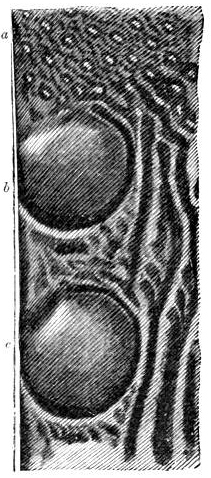
\includegraphics[width=4cm]{Proposal/ocelli.jpg}
\caption{The near summit portion of of male Argus pheasant's tail secondary wing-feathers, showing ball-and-socket ocelli and strips}
\label{fig:ocelli}
\end{wrapfigure}

As noted in \emph{The Descent of Man and Sexual Selection} \parencite{darwin1896descent}, animals and humans are often extravagantly ornamented. The crucial piece of evidence for sexual selection --- the ocelli and stripes of the male Argus pheasant's tail (Figure \ref{fig:ocelli}) --- is perhaps the most famous ornament in the animal world. Compared to Argus pheasants, the human body is rather dull, but the extended phenotypes --- the artefacts produced --- are not \parencite{Jones1856, Gombrich1994, Trilling2001}. While biological ornaments are frequently used for evolutionary studies, this project will focus on the decorative ornaments in the society --- ubiquitous and central to human culture, but often ignored \parencite{gluaveanu2014function}.\par
What is an ornament? It is typically composed of stereotyped sub-patterns, or \emph{motifs} \parencite{Gombrich1994, Trilling2001}, and adds qualitative features to objects alongside their quantitative states \parencite{sauglam2014re}. Motifs are recurring and repeated patterns with a consistent and distinct visual identity, they could be as simple as geometric, like Polka dots on fabrics, or as complicated as dragons on Chinese porcelains. In essence, they are cultural and aesthetic decorations designed to be reproduced with scale and through time. Ornaments are considered as important as language and counting to human beings, for they are how people make sense of the world, and they are the ``marks of humanity" \parencite{brett2005rethinking}. The way motifs are arranged in different ornaments can be considered as an ornamental style's grammar \parencite{Jones1856}, and the motifs themselves are its lexicon.\par
Cultural changes are much like organic evolution --- mutation vs novelty, tradition vs inheritance \parencite{Mesoudi2011}, and like how biologists study the evolution of animals through anatomy, one can study the evolution of cultures using ornaments. Evolutionary anthropologists are already using ornaments form Ikat weaving, Turkmen textiles, and Iranian carpets and their quantitative features to study cultural transmission and diversity from an evolutionary point of view \parencite{Tehrani2002, Tehrani2009, Buckley2012}. One can then estimate the rate of cultural evolution, and even study how drift and selection work in cultural populations \parencite{Lambert2017, leroi2020neutral}. Such studies open the gate of studying cultures using ornaments and their physical features. Although they present new possibilities for cultural studies, the identification and classification of motifs within ornaments are daunting due to its scale and complexity for scholars. Only between 1600 and 1800, the Dutch East India Company imported some 43 million pieces of Chinese and Japanese porcelain to Europe. Hundreds of thousands of them survive in public museums and private collections, and the diversity of their designs is vast \parencite{Campus2014}. Analysing such archives using the traditional way will require tons of domain experts, perhaps across several countries, and it would take them a reasonably long time --- hardly any project will have such luxury to do so. There is a lack of a more cost-efficient, perhaps computational method for finding the lexicon and grammar of ornaments. \par
This project aims to put together a computational method to study motifs and ornaments: the origins of all the patterns that fill our world, with a focus on Iznik. The choice of Iznik is made on the fact that they are immensely connected to the west and the east, the past and the present. From the 1480s onwards, artisans in Iznik, a town near Istanbul \parencite{necipouglu1989international}, began to produce lead-glazed fritware for the Ottoman court, with an apparent influence by the Chinese porcelains (Figure \ref{fig:Iznik_chinese}A), even though potters were unable to make porcelain properly \parencite{carswell1998iznik} at the time. By the mid-16\textsuperscript{th} century, it has developed its lexicon and started to have influences on other countries \parencite{canby2005islamic}. It is also at that time, local potters were sent to Damascus in Syria where they produced similar designs \parencite{Millner2015}. Iznik ceramics and their lexicon can be seen anywhere, from modern decorations sold in department stores, to the bottom of the North Atlantic on the wreck of \emph{RMS Titanic}.\par

\begin{figure}[H]
\centering
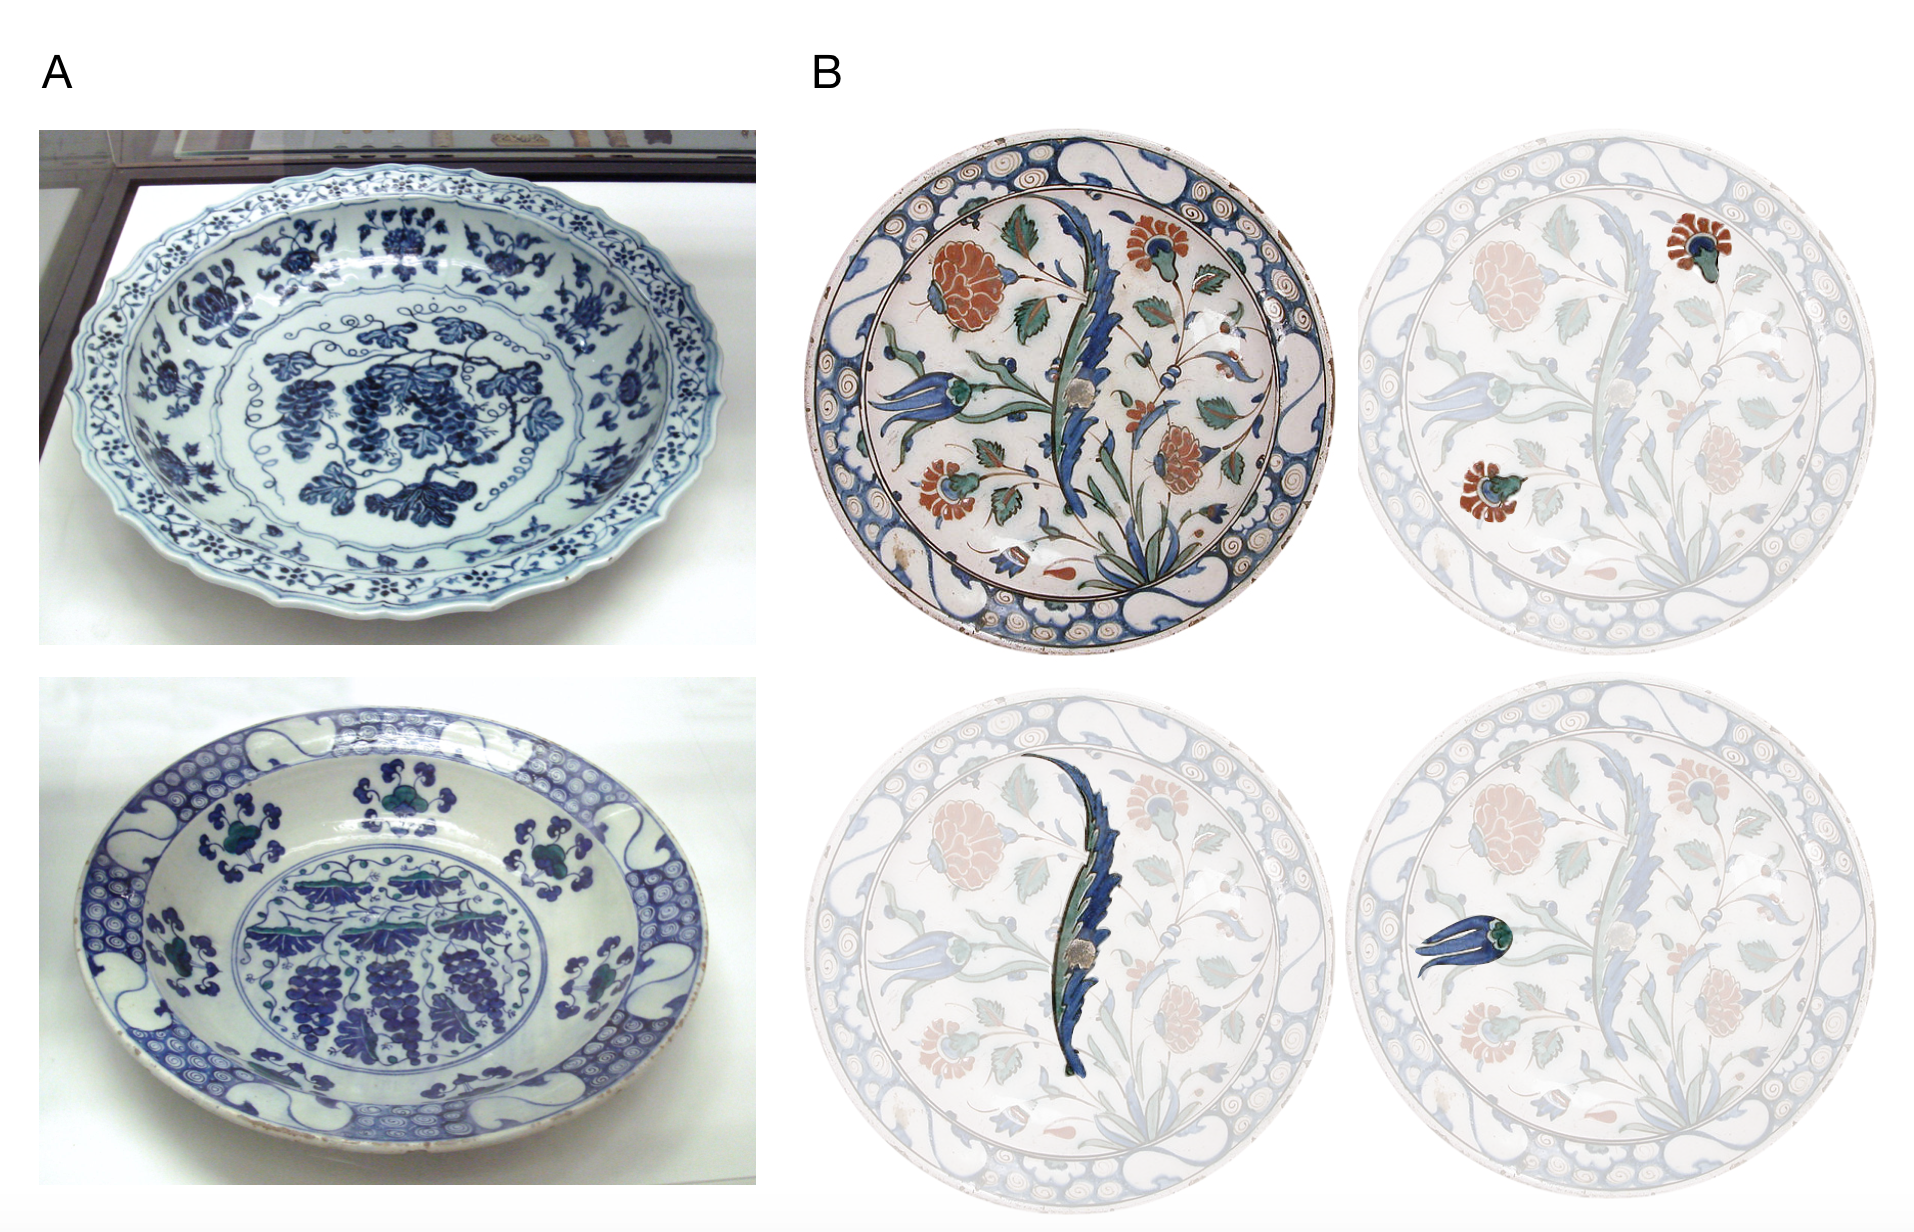
\includegraphics[width=10cm]{Proposal/Iznik.png}
\caption{An Iznik fritware and a Chinese porcelain in comparison. \textbf{A} Upper panel: Ming dynasty porcelain dish with grape design, Jingdezhen, China, 1403–1424; Lower panel: Fritware dish with grape design, Iznik, Turkey, 1550–1570; \textbf{B} A typical Iznik plate, with the three motif-families: tulip, carnation, and saz-leaf} 
\label{fig:Iznik_chinese}
\end{figure} 

This project chooses one of the most famous motif-families of the Iznik ornaments --- tulip (Figure \ref{fig:Iznik_chinese}B, bottom right) --- as an example of using computational methods to identify motifs. All tulips are clustered based on their colours, relative sizes and shapes using unsupervised methods. These clusters of tulips, or the motifs, then serve as the lexicon and form the foundation for understanding Iznik ornaments. A rarefaction analysis is also introduced on top of that to estimate the richness of motifs in the Iznik tulip. \par
With recent developments of computational, especially machine learning, tools, many scholars have been benefiting from implementing advanced technologies in their studies. Instance segmentation is a method typically used to identify and locate objects, along with masks (boundaries) from a given image. It has been widely used in medical imaging \parencite{pal1993review} and smart city applications like traffic control \parencite{shadeed2003road}. Recent applications of such methods, however, were applied to more diverse scenarios, ranging from identifying archaeological mounds using satellite image \parencite{orengo2020automated} to finding out the ripeness of strawberries at farms \parencite{yu2019fruit}. The same technique can be applied to the study of ornaments, helping with the tedious task of identification and classification of objects across different motif-families from images. For this project, a deep learning model for instance segmentation, Mask R-CNN \parencite{he2017mask}, is implemented to identify and classify objects of three motif-families --- tulip, carnation and saz-leaf (Figure \ref{fig:Iznik_chinese}B) --- automatically. 
Furthermore, because the instance segmentation model will be trained using objects from Iznik motif-families, holistically learning their features including the shape, pattern and colour, it should capture the overall ``style'' of Iznik motifs. So ideally, the model could also be used, as supplementary evidence, to help investigate how similar motifs from Iznik-style artefacts are to those of their Iznik ancestors based on its performance variations.\par
This study will explore on how to extract and analyse quantitative features of ornamental motifs; how well a deep learning model can do on extracting and classifying ornamental motifs; and whether the deep learning model trained on Iznik dataset can be used to study the similarity of other styles to Iznik. Collectively, these methods constitute a step towards the large-scale, quantitative analysis of the of ornaments, and in turn, cultures.\par

\section{Materials and methods}
\subsection{Data}
The dataset used for this project contained 575 images and was obtained from museum digital catalogues and monograph illustrations of Iznik artefacts (See Data and code availability). Among those images, 26.3\% were tiles, 62.1\% were plates, and the rest were tankards, jugs, vases, etc. (S.I. Table \ref{tab:artefacttype}). Images were then manually segmented into three different motif-families: tulip, carnation, and saz-leaf using expert's criteria (S.I. Defining motifs). 

\subsection{Lexicon discovery}
In order to have a better understanding of the tulip, only complete objects (that is, not fragmented or partially occluded) and those from good photographs (that is, were not unduly dark or oddly coloured) were used in this part of the project. In all, the lexicon discovery dataset consisted of 845 tulips from 320 images.

\subsubsection{Feature extraction: colour}
Although scholars generally speak with confidence of the colours of Iznik artefacts, in fact, any given colour comes in many different shades. In addition, the artefacts used in this project were photographed in many places and times without proper standards, so photography conditions add another source of colour variation. Given this, it is not an easy task to objectively assign colours to a given artefact. It is also unrealistic for experts to manually go through all images. For these reasons, two approaches were proposed to simplify each segmented object into a palette of the main colours used and their corresponding frequency. For that, both approaches require an overall palette built from the dataset, and all pixel values mapped to it. All analyses were done in the CIELAB colour space instead of RGB, as it is more perceptually linear than others, allowing a more accurate calculation in terms of colour differences \parencite{Luo2014}.\par
\textbf{Expert palette}.  
Melanie Gibson from Gingko Library Arts Series helped to identify 11 colours she thought were used and formulated the expert palette using randomly selected images from the dataset and her expertise in the subject. The expert then eyeballed major colours showed up on some new segmented objects, and estimated which colours on the expert palette they should belong to. This manually built colour map of some segments and the expert palette was then used as the training set for a supervised classifier to run through the whole set. (Figure \ref{fig: colpalflow} Expert palette). This top-down method is relatively static and requires some sort of expertise in the area. It also depends quite a lot on human judgements and manual works, which makes it less viable.\par
\textbf{Discover palette}.
Ideally, to generate a palette that indicates the nature of the colours in the segmented objects from artefacts, a bottom-up unsupervised clustering should be applied directly to all pixels. But clustering on every pixel is mostly impractical due to the huge amount of data. A sequential method was then proposed (Figure \ref{fig: colpalflow} Discover palette) to deal with this. Firstly, the final number of colours in this palette, $K$, was found. To do so, a series of 1\% pixel value samples of all segmented objects were obtained, and only the unique values were kept. Those values were then used for k-means clustering, with the $K$ set from 2 to 40. The clustering was done for 100 repetitions. The overall silhouette scores (S.I. Figure \ref{fig: silscore}) and within-cluster sum of square, WSS, (S.I. Figure \ref{fig: wss}) all indicated an optimal partition of just two colours but also a local optimum around $K$=10. To mirror with the expert palette, $K$=10 was used for this method. Each tulip then went through two layers of agglomerative clustering, with the same cut off of 20 colours to allow a fair amount of diversity. The first layer formed palettes of tulips based on their pixel values, and the second layer formed palettes of artefacts based on tulip palettes from the same image. After that, a layer of k-means clustering with the final $K=10$ on all palettes on artefact level was done to generate the discover palette. The procedure was adopted reasoning that the pixels of a given object, and the objects on a given artefact, would tend to be similar, that is, blue tulips on a single plate are probably the same blue. And because a lookup table is kept through the whole process, it is easy to accurately assign the final palette colour back to every pixel of the segmented objects.\par

\begin{figure}[H]
\centering
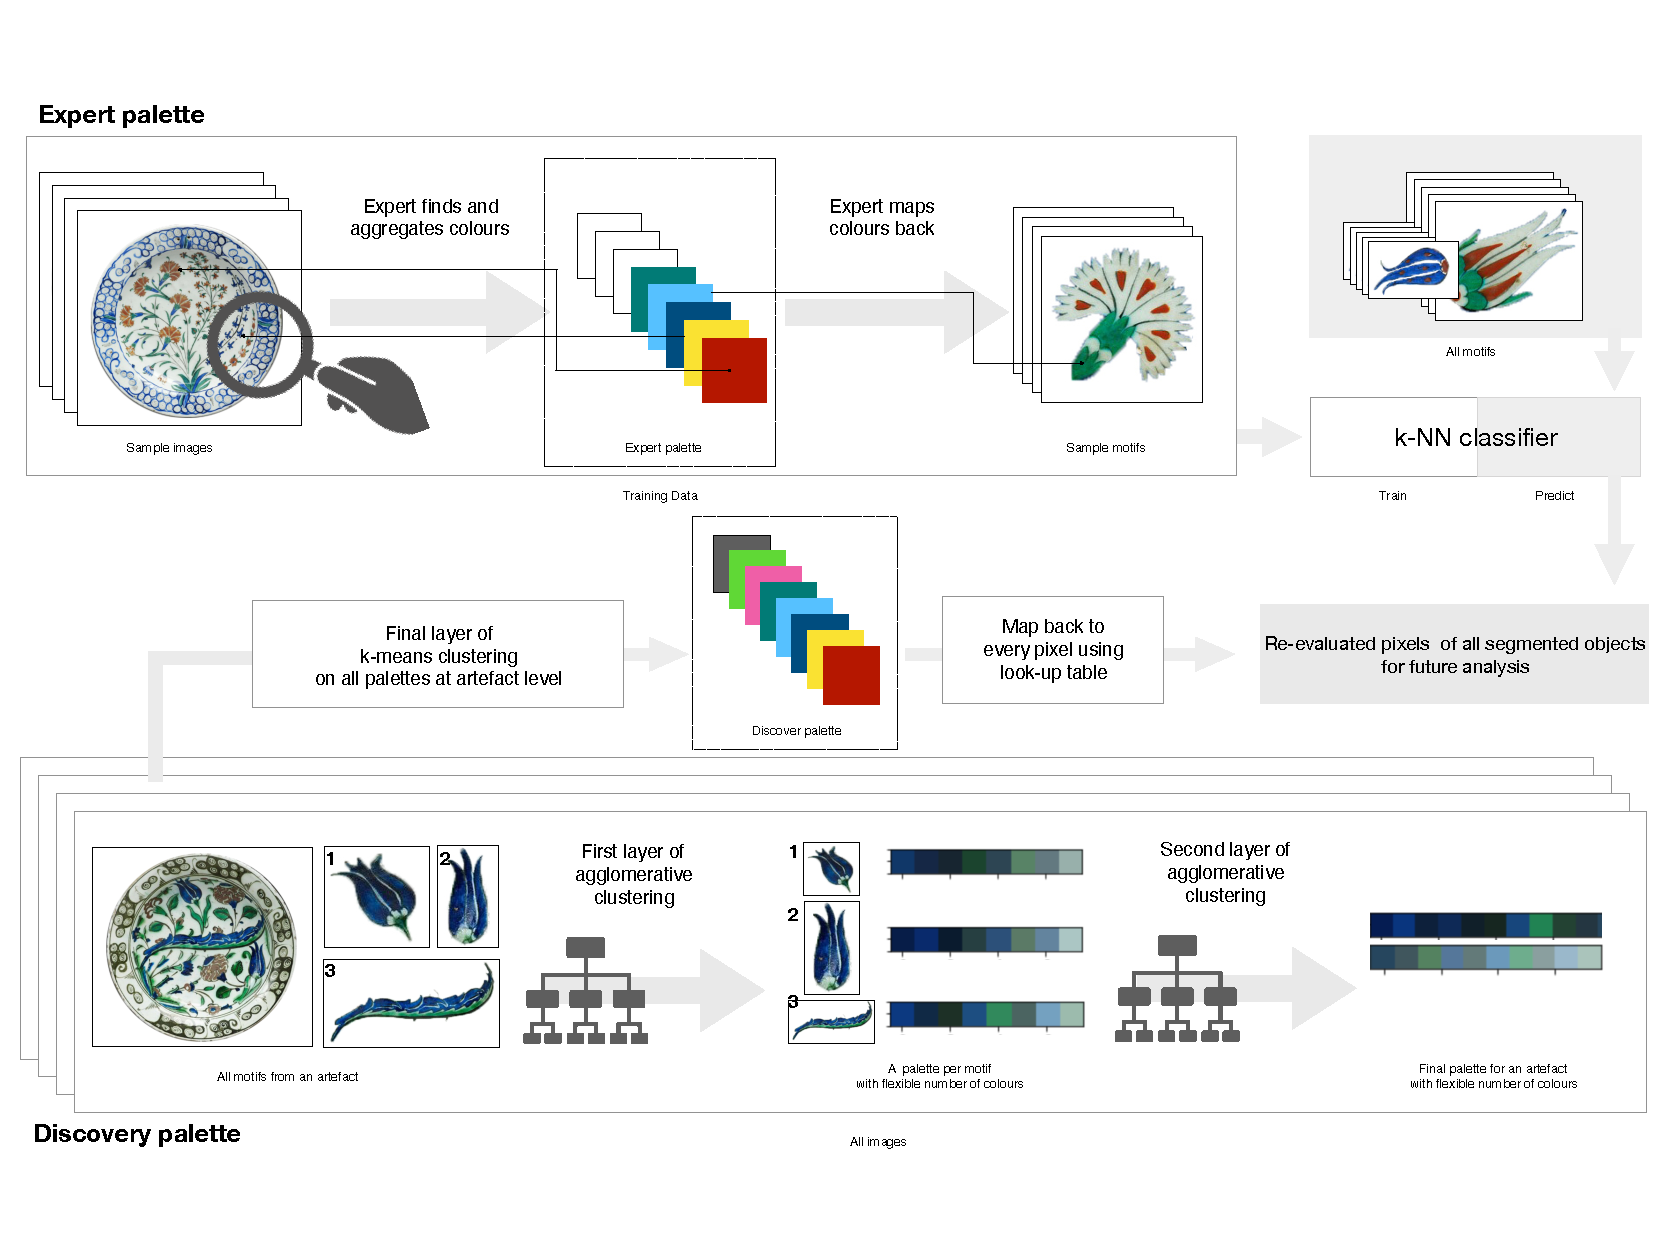
\includegraphics[width=15cm]{Proposal/colourpalflow.pdf}
\caption{Detailed workflow for obtaining the expert and discover palette. \textbf{Expert palette} Top-down method, from expert palette to re-evaluated pixels; \textbf{Discover palette} Bottom-up method, all pixels re-evaluated by three layers of clustering}
\label{fig: colpalflow}
\end{figure}

\subsubsection{Feature extraction: shape and size}
The following methods were applied to each of the segmented tulips to obtain their geometrical features.\par
\textbf{Shape}.
Each object in the dataset was manually segmented and placed against a white background. Outlines of the tulips were extracted and re-sampled into evenly-spaced, size-standardised, lightly-smoothed coordinate sets. Alignment of the object coordinate sets was done using the following steps: (i) randomly selected an object as the reference; (ii) rotated each object outline in a given family sequentially through 360\textsuperscript{o}, with a step of 1\textsuperscript{o}; (iii) for each image rotation, the distance of the coordinates to the reference subject were calculated, and the one the with the shortest distance and the most correlated y is chosen to be the aligned object. The final result was a collection of outlines, one per object, with the same orientation (S.I. Figure \ref{fig:alignment}). Principal Components Analysis, PCA, were carried out on re-aligned outlines after standardisation. \par
\textbf{Size}.
The area (pixels taken up) of each object relative to the artefact it's on was used as a measure of size. In the case of tiles, which often come in panels, an estimation of the object size relative to a single tile was used. \par

\subsubsection{Spectral clustering}
The previous colour, shape, and size descriptors were used to study the lexicon of Iznik tulips. Spectral clustering was chosen due to its flexibility. Clusters are not assumed to be any certain distribution for this method, contrary to k-means, meaning this algorithm can perform well with the wide variety of the data used. The traditional eigengap method was not used to find the optimal $K$ for this clustering practice. Instead, a method that examined the multimodality of the eigenvectors was implemented to work with potential nonGaussian structures in this task \parencite{john2020spectrum}. In the end, the cluster results of each feature would collectively form the lexicon of the tulip. \par

\subsubsection{Rarefaction analysis}
The results from clustering analysis could serve as abundance data, illustrating each motif's occurrence in Iznik tulips. Assuming the distribution of motifs in tulips is random, or relatively close to the reality, a rarefaction analysis could provide a snapshot and prediction of its species richness. In brief, the rarefaction analysis works by sequentially drawing objects from a pool and asking whether it is a new motif. Initially, the number of new motifs increases steeply but then asymptotes as all motifs have been already enumerated. The observed samples of abundance were used to compute diversity estimations and the 95\% confidence intervals using functions developed in \cite{rarearticle}.

\subsubsection{Tools}
All analyses and data handling in this part were carried out using \texttt{Python 3.6} and \texttt{R 3.6.1}. For the colour palette part, \texttt{class} in \texttt{R} was used for the supervised classifier, \texttt{Python} package \texttt{sklearn} was used for the sequential clustering method, and calculating the optimal $K$. 
Data preparation including getting the object contour and re-sampling were done with \texttt{Python} package \texttt{skimage} and \texttt{numpy}, while the alignment, PCA, and spectral clustering were done with \texttt{R} package \texttt{Momocs}, \texttt{princomp} and \texttt{Spectrum} respectively. The rarefaction analysis and estimation were conducted using \texttt{iNEXT} \parencite{inext} in \texttt{R}.


\subsection{Instance segmentation}
This part of the project ended up using 575 images, manually segmented for three families of motifs: carnation ($N=504$), tulip ($N=2,045$) and saz-leaf ($N=1,756$).\par

\subsubsection{Data pre-processing}
The manually prepared dataset contains images of artefacts and their corresponding cut-off motifs. Although cutting them out was a labour-intensive task, it laid the foundation for incorporating machine learning tools for data gathering of such. Mask R-CNN is a well-known model for computer vision tasks, especially for instance segmentation. Two metadata were added to the dataset: coordinates of polygons (masks) covering the instances themselves, which were already obtained from the previous shape analyses, and coordinates of bounding boxes indicating the rough area of each instance, which were estimated using the shape coordinate sets. The dataset was then transformed into the COCO annotation format \parencite{lin2014microsoft}. Images, and their corresponding metadata were randomly split into two groups with a ratio of 9:1 for training and testing, respectively. The training and evaluation of the model were performed three times. Details of the training and testing set of each repetition can be seen in S.I. Table \ref{tab:repetition}.\par

\subsubsection{Model evaluation}
Average Precision, $AP$, and Average Recall, $AR$, were used to examine the result's relevancy, and the ability of the model to find all relevant cases within the dataset. 
To do this, a ranking of all predictions by their prediction score, $s_{p}$, was made. An intersection over union, or $IoU$, the threshold at which to estimate $AP$ was also set. $IoU$ (Figure \ref{fig:iouauc}A) is a metric of the degree to which a prediction overlaps with its corresponding ground truth, and varies between 0 (no overlap) and 1 (complete overlap). An $IoU$ is calculated as:
\begin{equation}
IoU=\frac{M_p\cap M_g}{M_p\cup M_g}
\end{equation}
where $M_p$ and $M_g$ are the set of pixels that occur in the predicted and ground truth masks, respectively. Given some $IoU$ threshold, each prediction is then judged to be either a true or false positive. \par
The precision and recall pairs over all ranked predictions are calculated as:
\begin{equation}
Precision = \frac{N_{T}}{N_{P}}\\
\end{equation}
\begin{equation}
Recall = \frac{N_{T}}{N_{G}}\\
\end{equation}
where $N_{T}$, $N_{P}$, $N_{G}$ are the counts of true positives, predictions and ground truth for any $IoU$ threshold and rank in the list of predictions. A precision-recall curve (Figure \ref{fig:iouauc}B) can be built using these pairs.\par
Each dropping of recall on the curve, $r_i$, is sampled, and $AP$, then, is the area under this curve:
\begin{equation}
AP = \sum (r_{n+1}-r_n)P_{interp}(r_{n+1})\\
\end{equation}
where
\begin{equation}
P_{interp}(r_{n+1}) = \max_{\widetilde{r}\geq r}p(\widetilde{r})\\
\end{equation}
For the evaluation, $AP$s for $IoU$ thresholds of 0.5, 0.75 and 0.5-0.95 using 0.05 size bins were calculated and referred respectively as $AP_{0.5}$, $AP_{0.75}$ and $AP_{0.5-0.95}$, while average recall was only calculated using the thresholds of 0.5, and 0.5-0.95 range as $AR_{0.5}$, and $AR_{0.5-0.95}$.

\begin{figure}[H]
\centering
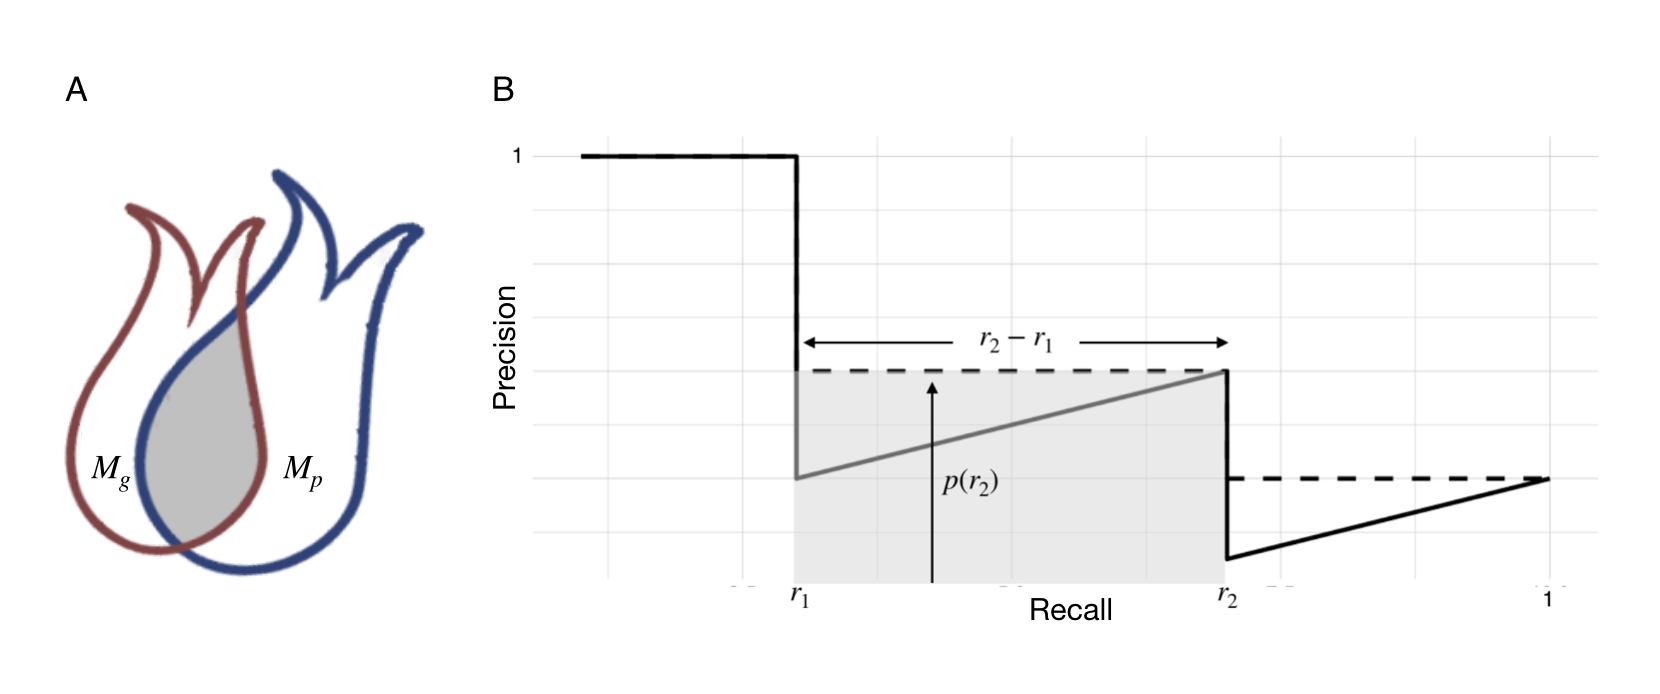
\includegraphics[width=14cm]{Proposal/iouauc.png}
\caption{Metric details for model evaluation. \textbf{A} Definition of $IoU$ (where the gray area is the intersection, and overall is the union); \textbf{B} A typical precision and recall curve with a interpolated precision}
\label{fig:iouauc}
\end{figure}


\subsubsection{Configurations and tools}
The segmentation model was based on the Mask R-CNN implementation on Detectron2 \parencite{wu2019detectron2} and PyTorch \parencite{NEURIPS2019_9015}. A pre-trained weight was used with ResNet-50 \parencite{ he2016deep} and FPN \parencite{lin2017feature} backbone as the baseline, as it obtained the best speed and accuracy trade-off across all available weights. Weights were trained on the MSCOCO 2017 train/val dataset and provided by the Detectron2 API. The final base learning rate was set to 0.02, which gave an optimal performance. The other training parameters were chosen to match the machine's hardware capacity (Table \ref{tab:segmethods}).\par

\begin{table}[H]
\centering
\caption{Configurations of the instance segmentation task, image augmentation was done during the training using Detectron2 built-in functions.}
\begin{tabular}{lc}
\hline
Parameter & Value\\
\hline
Number of classes & 3\\
Backbone & ResNet-50, FPN\\ 
Images per batch & 4\\ 
Base learning rate & 0.02\\ 
Batch size per image & 512\\
Maximum iterations & 25000\\ 
Augmentation & ResizeShortestEdge, RandomFlip\\ 
\hline
\end{tabular}
\label{tab:segmethods}
\end{table}

This part of the project was done solely in \texttt{Python 3.6}, with \texttt{Torch 1.5}, \texttt{Detectron2 0.1.3}, and \texttt{COCO} API was used for the instance segmentation training and evaluation. \texttt{numpy} and \texttt{json} were used for most of the pre-processing. Model training and inference was done on a single NVIDIA Tesla P100 GPU.\par

\subsection{Similarity of other stylistic traditions to Iznik}
For this particular task, the ability of the model to identify tulips in other traditions was tested. Tulips were chosen because the model is good at finding them in Iznik, and also because one of the ornamental tradition to examine is rich in them: 17\textsuperscript{th} century Dutch Delft. Details of the data used for this part of the project are shown in Table \ref{tab:similaritytest}.\par
\begin{table}[H]
\caption{Details of data used for testing similarity of other stylistic traditions to Iznik ceramics}
\small
\centering
\begin{tabular}{cp{3cm}p{3cm}cc} 
\hhline{~----}
 & Date & Area & Tulip & Image count \\ 
\hline
ICAROS & 1930-1988 & Rhodos & 176 & 26 \\ 
Northern European factories & 19\textsuperscript{th}-20\textsuperscript{th} centuries & Northern European  & 70 & 25\\ 
Dutch Delft & 17\textsuperscript{th} century & Delft & 47 & 32\\ 
\hline
\end{tabular}
\label{tab:similaritytestdata}
\end{table}
A looser $IoU$ threshold of 0.5 was used since none of the segmented objects were to be used for in-depth analysis of their shapes or colours. $AR$ and $AP$ at this particular threshold were used to compare the model's performance on different stylistic datasets and on Iznik. The idea is that, by examining how many objects the model could find using features learned from the Iznik training data, the similarity of different styles to Iznik can be measured more or less.\par 

\section{Results}
\subsection{Lexicon discovery} 
The lexicon discovery part was focused on Inzik tulips (Figure \ref{fig:Iznik}), and the result here gives a general idea of how well it worked.
\begin{figure}[H]
\centering
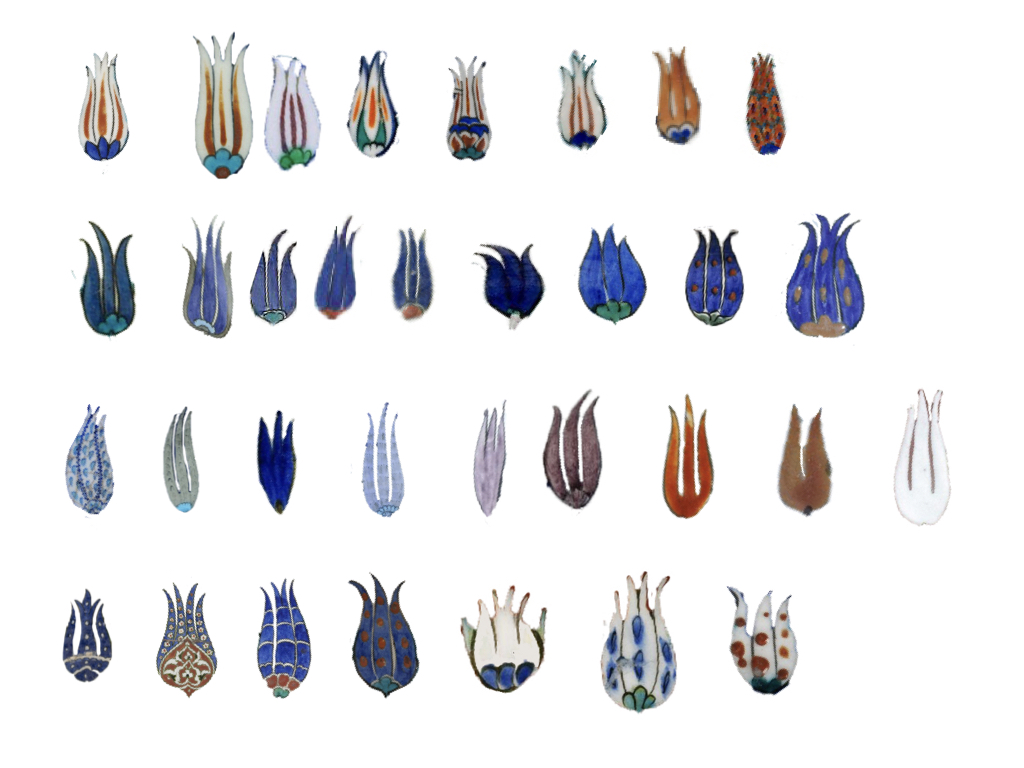
\includegraphics[width=10cm]{Proposal/tulipcol.jpg}
\caption{Examples of Iznik tulips, manually segmented from artefact images} 
\label{fig:Iznik}
\end{figure} 
\subsubsection{Comparison of two colour palettes}
Although the expert palette clearly captured the major colours used by Iznik artisans, experts had issues when aggregating colours together, struggling to maintain a consistent level of abstraction (S.I. Table \ref{fig:expertpalproblem}). The palette unconsciously emphasised rare colours like purple. And these not-yet-needed details were not helpful for the task of understanding the overall style. It also ignored variations (caused by the composition of the pigment, how it was applied, the firing conditions of the artefact, etc.) within a general colour and it required expert knowledge to maintain and update. Hence the expert palette is not always viable for such analyses. Figure \ref{fig: palette} shows that the discover palette, compared to the expert one, takes up a relatively similar colour space. Considering the discover palette is flexible (relatively easy to adjust the palette's granularity based on the number of colours used), easy to implement (requires only images), and reflecting the reality of the colour (analysed with good quality images), it was used for the rest of the project. Frequencies of the discover palette colours in each object were calculated and used for future analysis.\par

\begin{figure}[H]
\centering
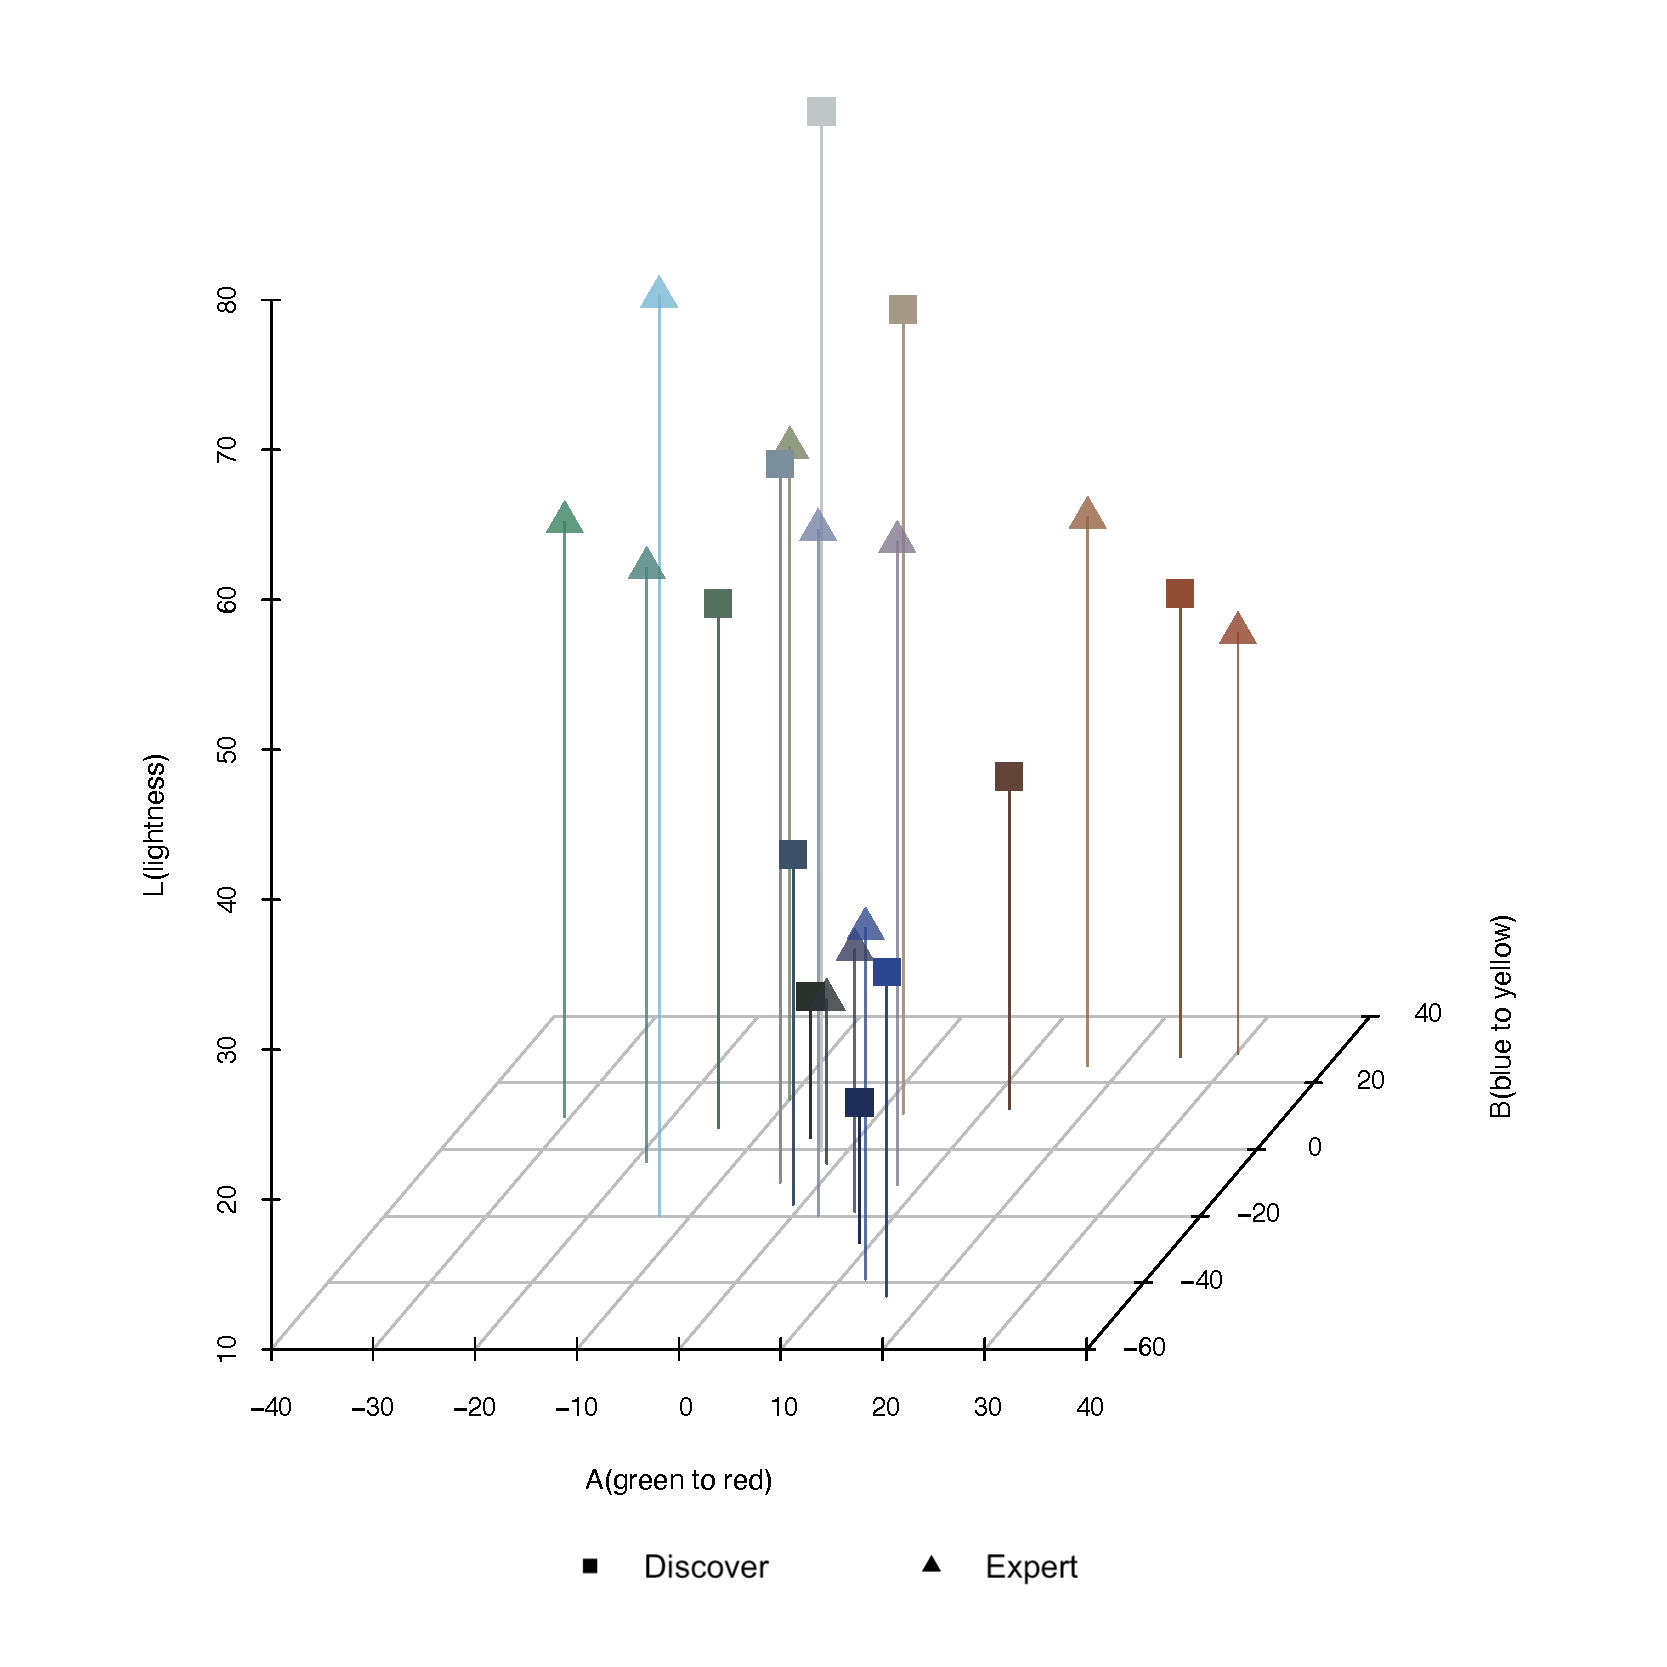
\includegraphics[width=14cm]{Proposal/palette.pdf}
\caption{Expert and discover palette of Iznik artefacts in CIELAB space. Colours on the figure correspond to actual colours in the palette}
\label{fig: palette}
\end{figure}

\subsubsection{Lexicon of tulips}
The analysis on the shapes of tulips was done based on the first 25 PCs obtained, which account for 99\% of the variance. A plot of tulips using the first two PCs (Figure \ref{fig:tulippc}) shows the approach was effective. The tulips on the bottom part of the graph have mostly three longer petals, while the tulips at the top mostly have two shorter ones. There is also a trend for the shapes of tulips to be more abstract (more realistic to oval-like shape) from the bottom left to the top right.\par
\begin{figure}[H]
\centering
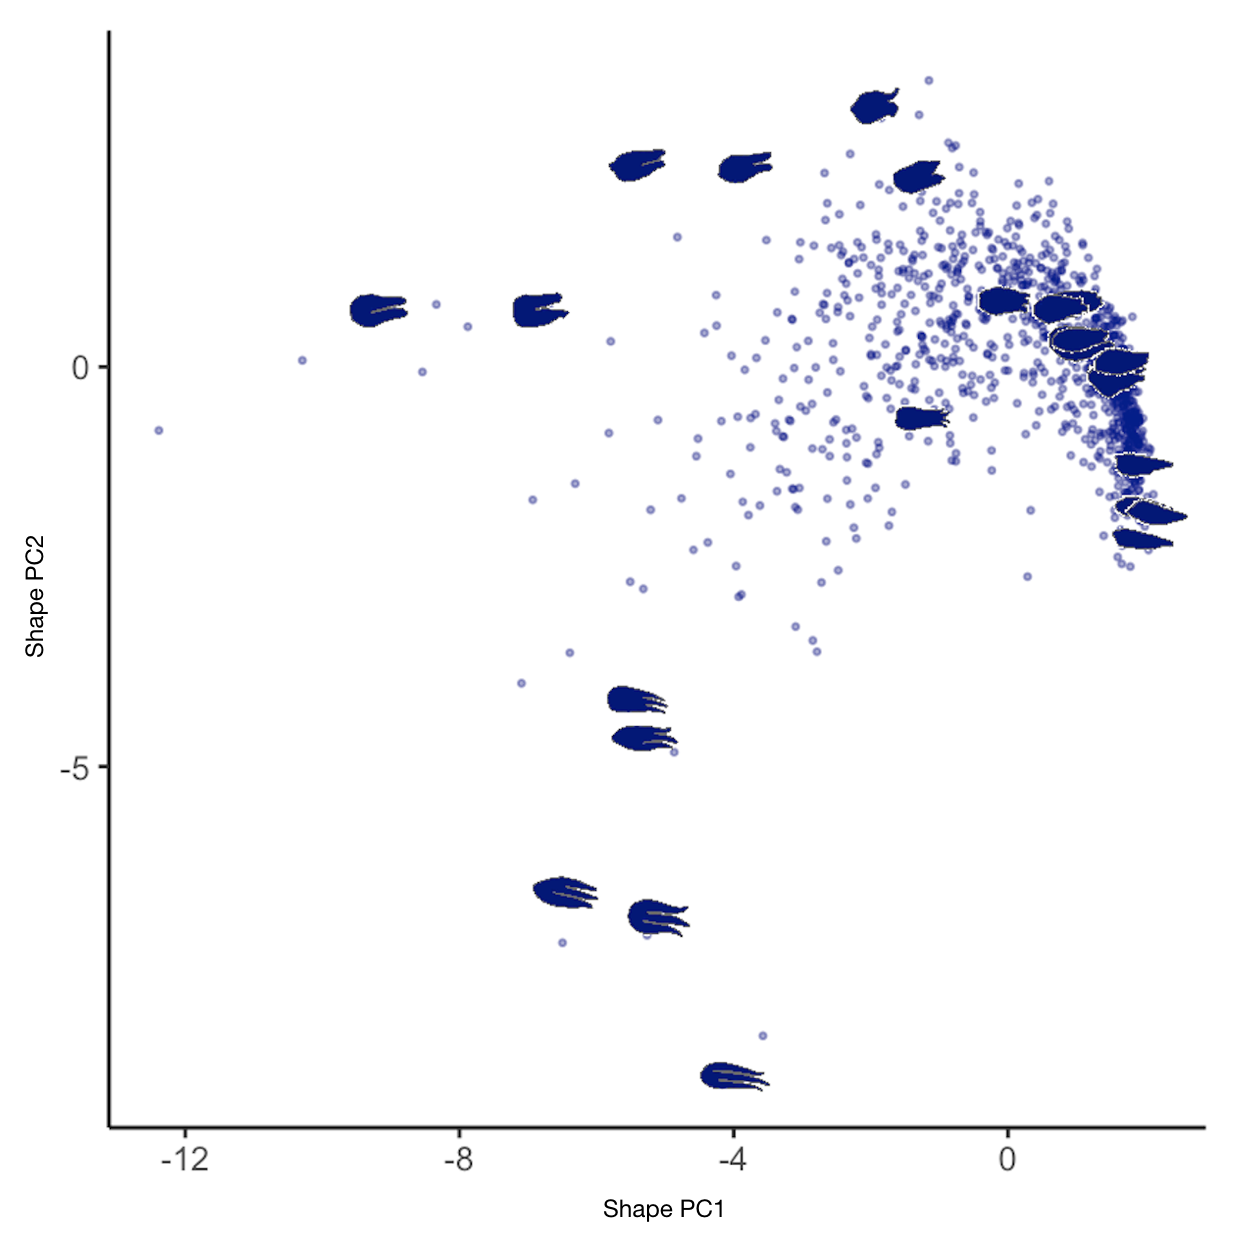
\includegraphics[width=16cm]{Proposal/tulips_pcplot.png}
\caption{Distribution of tulips using the first two PCs. Random samples of the points are taken and corresponding tulip shapes are plotted as well. As can be seen in the graph, PC1 represents how open or closed these tulips are, and PC2 represents how complex the openings are}
\label{fig:tulippc}
\end{figure}
These shape PCs, along with the colour frequency data (calculated using the 10 colours from the discover palette) and relative sizes were then used for clustering. The spectral clustering gave 4 clusters in shape (see details in S.I. Figure\ref{fig:clustershape}), 10 clusters in colour(see details in S.I. Figure\ref{fig:clustercolour}), and 3 clusters in size. Collectively, these clusters theoretically created 120 unique motifs in the tulip family (Figure \ref{fig:clusterresults}), whereas in the dataset, 68 of them appeared. On average, each artefact from the dataset has 5.5 tulips on them, and has 2.3 motifs in total.\par
\begin{figure}[H]
\centering
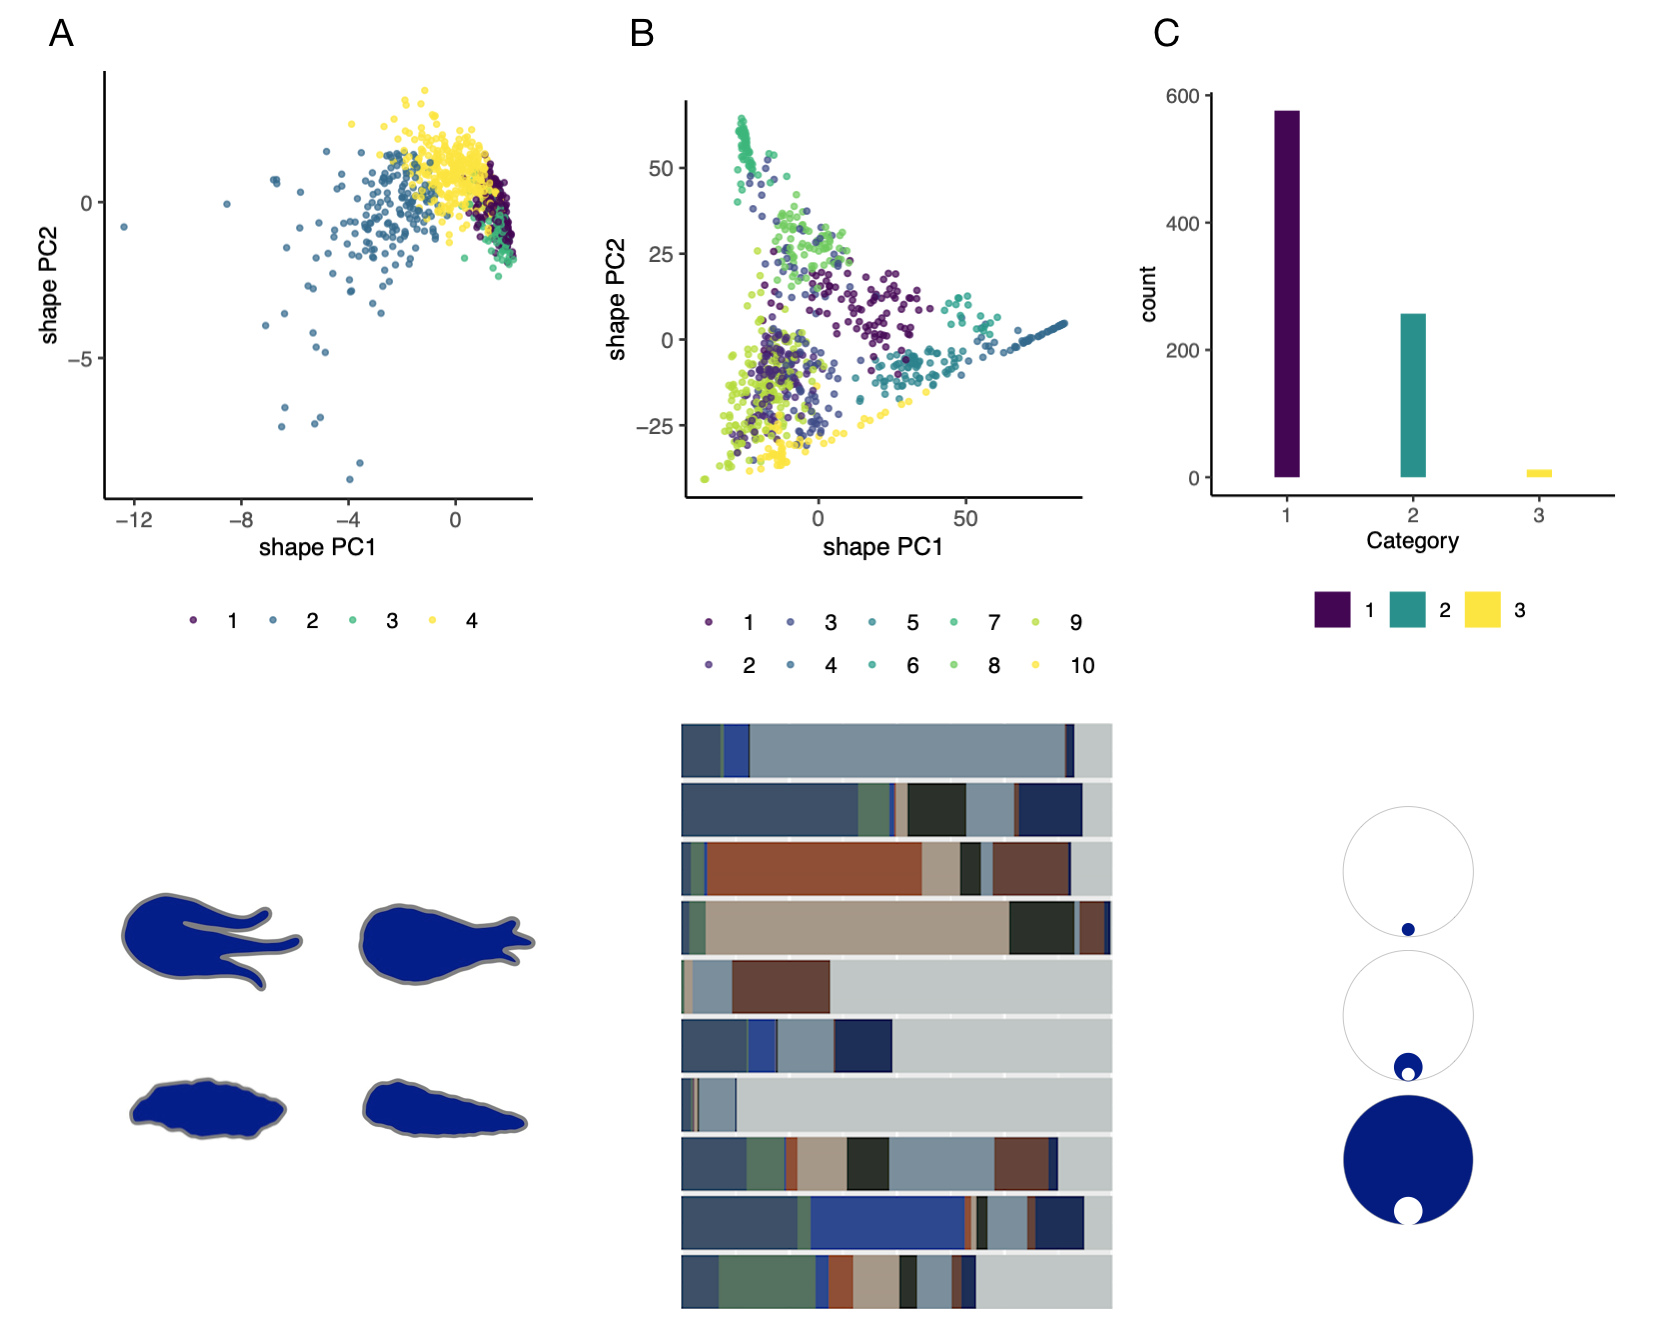
\includegraphics[width=13.5cm]{Proposal/clusterresults.png}
\caption{Cluster results on shape, colour, and size. \textbf{A} 4 clusters in Shape. Top panel, cluster results in scatter plot. Bottom panel, typical shapes in the 4 clusters; \textbf{B} 10 clusters in colour. Top panel, cluster results in scatter plot. Bottom panel, mean colour palettes from the 10 clusters; \textbf{C} 3 clusters in size. Top panel, Histogram of cluster distribution. Bottom panel, motif area $\leq 1\%$,  $1\% <$ motif area $\leq 5\%$, and motif area $> 5\%$ }
\label{fig:clusterresults}
\end{figure}
A rarefaction analysis was done on the 845 tulips of 68 unique motif types (species) to understand the species richness of Iznik tulips. The curve reaches the plateau phase at sample size around 500, and estimates there to be about 70 kinds of tulip motifs (Figure \ref{fig:rare}) in the Iznik ornamental lexicon. Each of the motifs comes in a variety of forms which, to continue the linguistic metaphor, resembles the spelling or pronunciation variants. The analysis showed that nearly all tulips were discovered using this method.   
\begin{figure}[H]
\centering
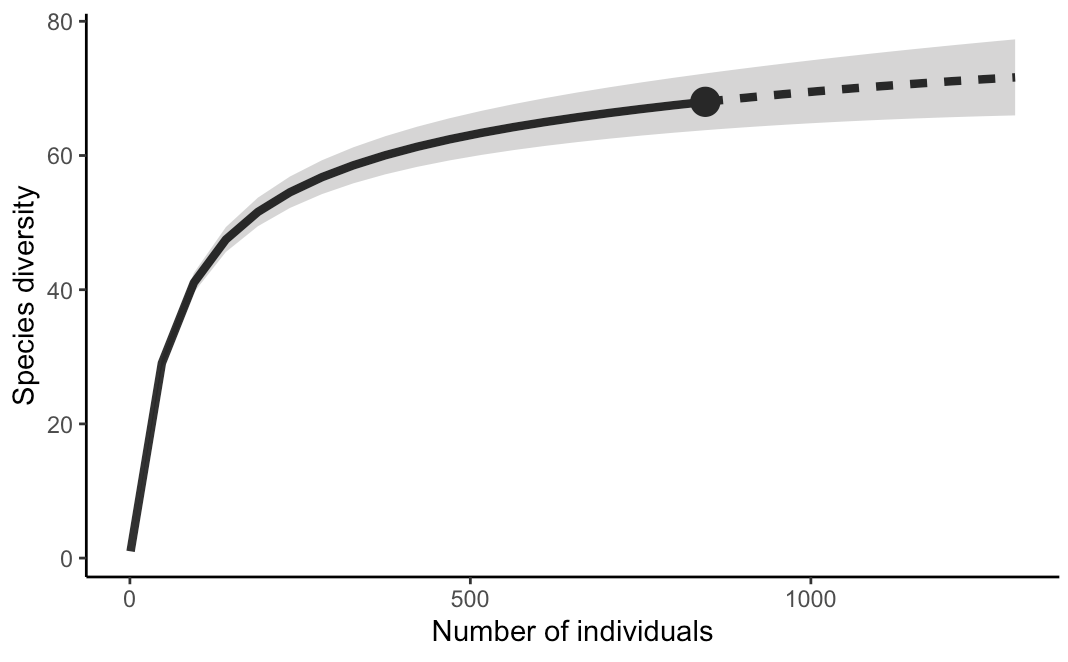
\includegraphics[width=9cm]{Proposal/rare.png}
\caption{Rarefaction curve, with estimation, of motifs within Iznik tulips drawn with cluster results. Step of sampling set to 20, and shaded with 95\% confidence intervals}
\label{fig:rare}
\end{figure}
\subsection{Instance segmentation}
In this part of the project, the ability of a wildly-used deep learning model --- Mask R-CNN --- to automatically segment motifs out of ornamental objects was tested. The model was initially based on weights trained on a standard segmentation dataset and then fine-tuned to find all three motif-families --- tulip, carnation and saz-leaf --- on images of artefact from the entire dataset ensure good coverage. \par
In order to test whether the model performed in a consistent way, three repetitions were done using the same configuration. For each repetition, 60 images (\~10\%) of the dataset were randomly selected to be the test set, and the model was trained on the remaining 515 images. Figure \ref{fig:eval} shows the overall precision-recall curves for each repetition at an $IoU$ threshold of 0.5. The Coefficient of Variation, ${\widehat {c_{\rm {v}}}}$, of the $AP$s was calculated as:
\begin{equation}
{\widehat {c_{\rm {v}}}}={\frac {s}{\bar {x}}}
\end{equation}
where $s$ and $\bar{x}$ are standard deviation and mean of the $AP$s.\par
\begin{figure}[H]
\centering
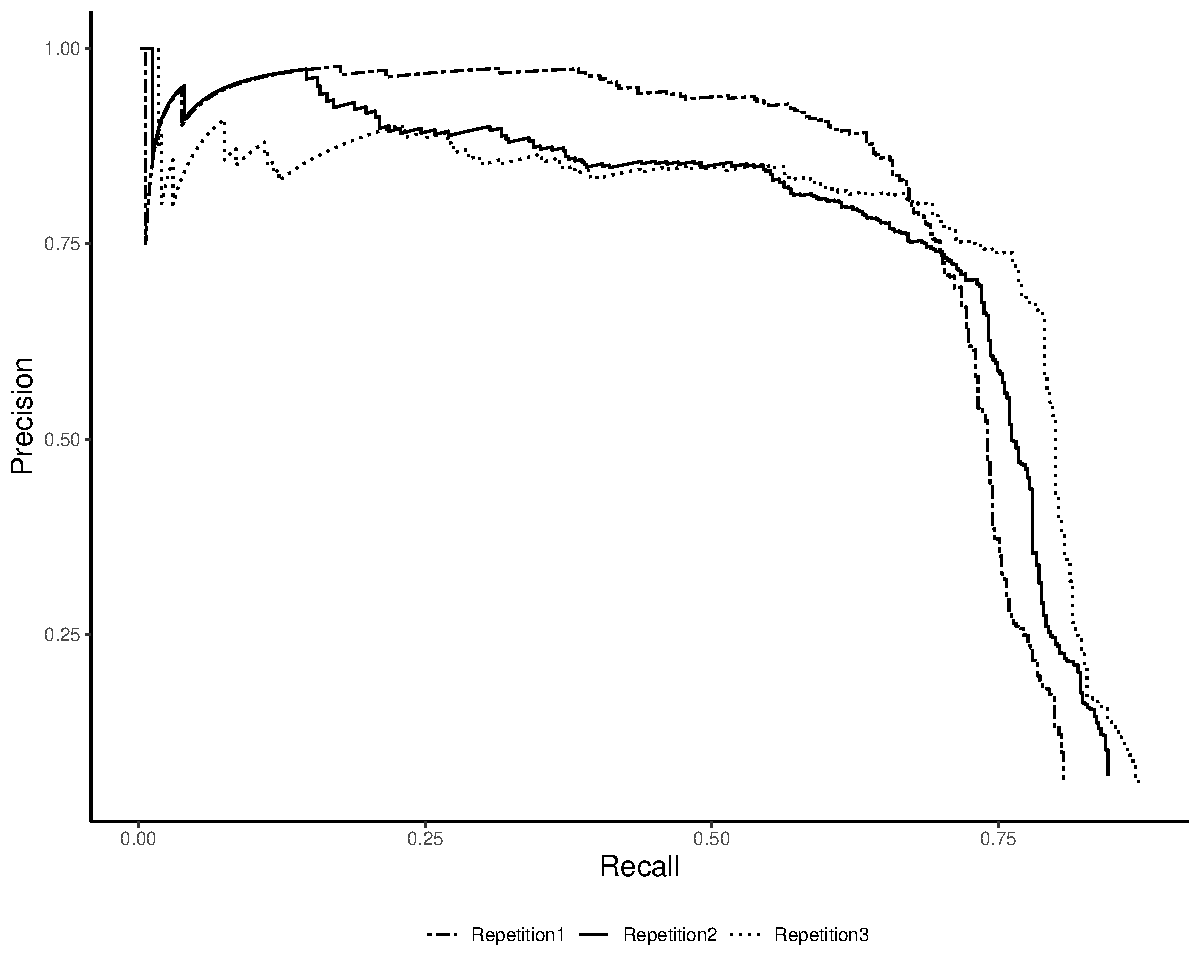
\includegraphics[width=12cm]{Proposal/PR_curves.pdf}
\caption{Precision-recall curves using $IoU$=0.5, for the three repetitions.}
\label{fig:eval}
\end{figure}

The $AP$s of the three repetitions has a $CV$ of 0.03, which is smaller than 1, meaning it is a relatively low-variance distribution and the model behaved consistently.\par
Each prediction in each repetition located a putative object in an image with a mask, and identified motif-family to which it belongs to, and had a prediction score that tells us how good the model thinks it is. Figure \ref{fig:segmented}A shows four tulips on a plate from the Ashmolean successfully predicted by the model. To evaluate the model, the Average Precision, $AP$, and Average Recall, $AR$, of predictions in each repetition were calculated. It is necessary to specify a criterion, $IoU$, by which a given prediction is deemed as acceptable to get the $AP$. Table \ref{Tab:AP} reports the $AP$s for two thresholds: $IoU$=0.5, 0.75, and the $AP$ and $AR$ for all $0.5 \geq IoU \leq 0.95$ across three repetitions. The curves are close to the right top corner meaning the model is behaving well. Overall, the model has a mean $AP_{0.5}$=72.0, $AP_{0.5-0.95}$=53.3, and $AR_{0.5-0.95}$=74.8. Using similar methods, \cite{zhao2018comparing} achieved an $AP_{0.5-0.95}$=57.5 on finding pomegranate tree canopy from aerial images, \cite{toda2020training} achieved an $AP_{0.5-0.95}$ around 50 on finding seeds from a single colour background, while \cite{8759574} achieved an $AP_{0.5-0.95}$=50.8 on finding neuropathic ulcers. The model of this project performed at the same level as those mentioned above. However, it is noteworthy that their tasks were simpler in the sense that they were finding single category items on relatively clear backgrounds, where this project identified multiple categories on complex backgrounds. It can be seen that the model was better at segmenting some motif-families than others. While it was able to segment tulips and carnations with relatively better performance, it was not as good when dealing with saz-leaves.\par


\begin{table}[H]
\centering
\caption{Mean Average Precision, $AP$, and mean Average Recall, $AR$, with standard deviation from the three repetition for the test set of 60 images assuming different $IoU$ thresholds, specified by subscript.}
\begin{tabular}{lcccccc}
\hhline{~~-----}
& & \multicolumn{3}{c}{$AP$} & \multicolumn{2}{c}{$AR$} \\ 
\hhline{~~-----}
& & $AP_{0.5}$ & $AP_{0.75}$ & $AP_{0.5-0.95}$ & $AR_{0.5}$ & $AR_{0.5-0.95}$\\ 
& & Mean(SD) & Mean(SD) & Mean(SD) & Mean(SD) & Mean(SD) \\ 
\hline
Tulip & & 73.7(3.08) & 68.7(4.53) & 55.7(3.37) & 87.0(4.62) & 81.4(3.51)\\ 
Carnation & & 79.6(5.56) & 73.7(8.37) & 63.4(6.88) & 88.8(2.00) & 77.7(7.13)\\ 
Saz-leaf & & 62.8(3.94) & 48.8(2.32) & 40.9(1.91) & 79.5(3.48) & 65.2(0.75)\\ 
All categories & & \textbf{72.0}(2.05) & 63.7(3.85) & 53.3(2.91) & \textbf{85.1}(3.20)& 74.8(2.14)\\
\hline
\end{tabular}
\label{Tab:AP}
\end{table}

\begin{figure}[H]
\centering
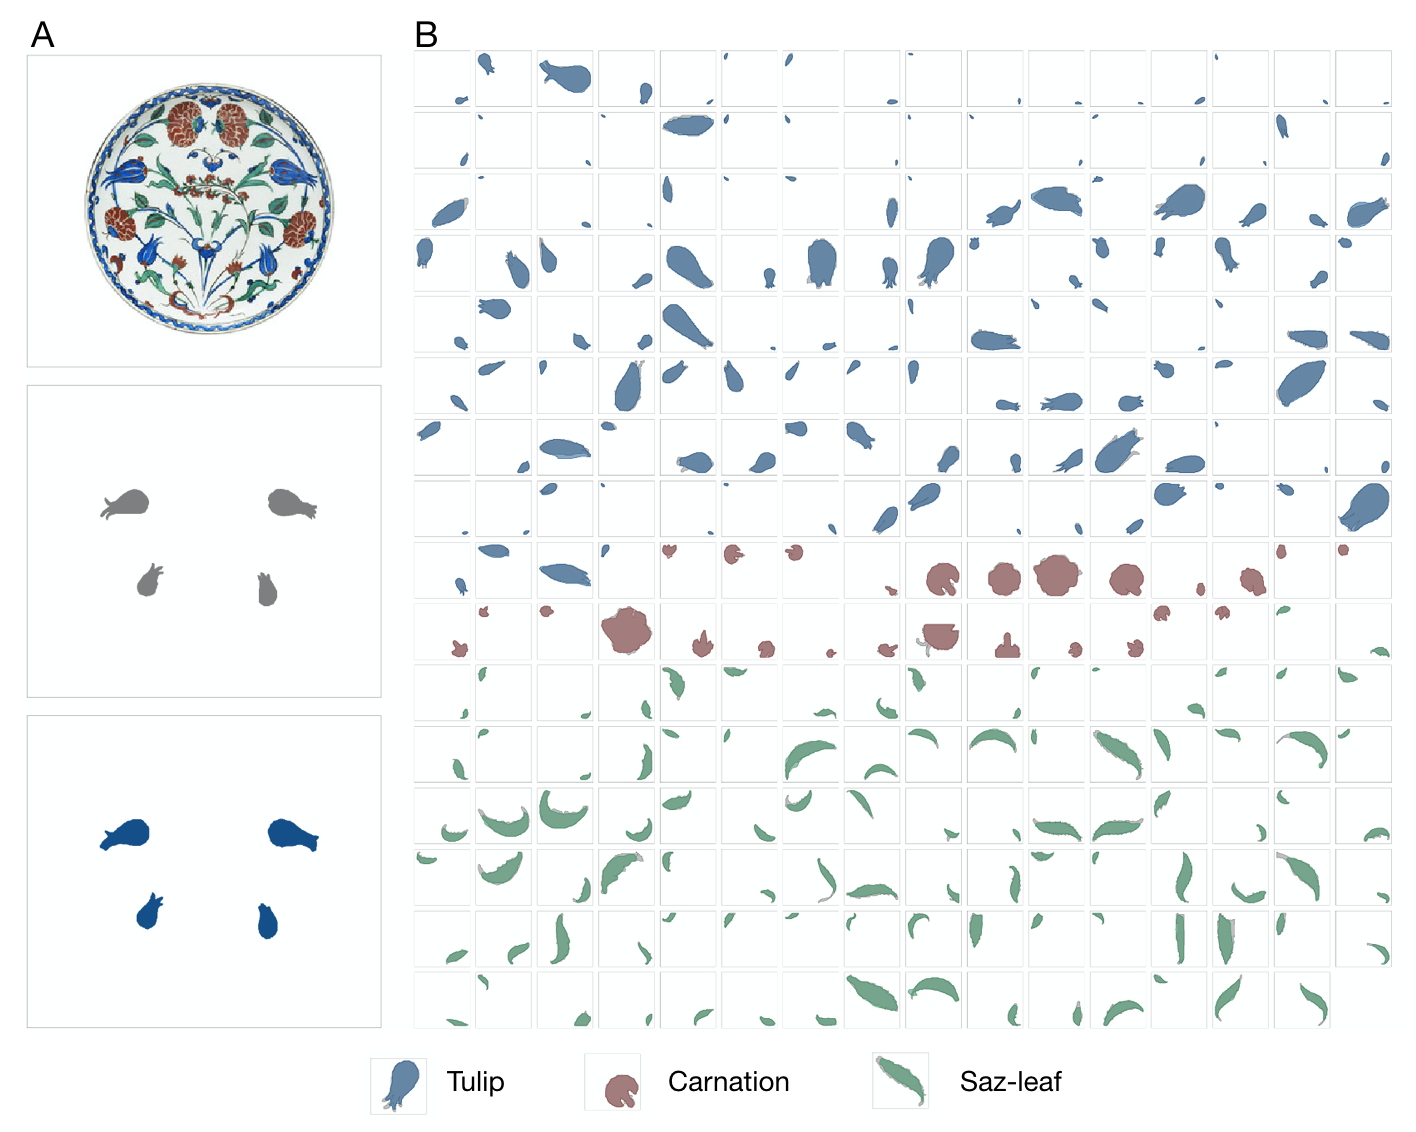
\includegraphics[width=13cm]{Proposal/Figure_X_segmentation.png}
\caption{Segmentation of ornamental objects by Mask R-CNN \textbf{A} A successful example. Top panel, a plate from the Ashmolean containing four tulips. Middle panel, manually isolated ground truth objects. Bottom panel, objects predicted with score $s_{p} > 0.9$; \textbf{B}. Successfully segmented objects from the Iznik test set. Predictions filtered by prediction score $s_{p}>0.075$ and $IoU \geq 0.75$; ground truth in grey overlain by coloured prediction}
\label{fig:segmented}
\end{figure}
How useful is the deep learning model? Since the objective here is to get the most out of the prediction, meaning to obtain as many qualified predicted objects as possible, $Recall$, prediction score $s_{p}$, remaining prediction percentage $p_{p}$, and $IoU$ are used for understanding the behaviour of the model in action. Suppose an entirely new set of 1,000 artefact images were obtained. Keeping the distribution of motifs on these new images same as the previous dataset, it will give about 8,441 tulips, carnations and saz-leaves in total, and the model will produce around 100,000 predictions. By setting a threshold of predicting score, $s_{p}$, most, but not all, poor predictions can be filtered out. For example, if a filter at $s_{p}\geq0.075$ were set, only 75\% of the total segmented objects will be covered by those predictions($Recall=75$), and only about 8\% of the predictions will remain ($p_{p}=7.8\%$). Since the result will most likely be used for morphological analysis, a stricter $IoU$ threshold of 0.75 is used for more accurate results. Given these settings, the $Recall$ is calculated to be 59, meaning the model will cover around 60\% of the total objects appeared on the new dataset. A detailed $p_{p}$, $Recall$ curve (S.I. Figure \ref{fig: recall}) based $s_{p}$ tell more about the trade-off between prediction count and object covered by prediction. Figure \ref{fig:segmented}B shows a snapshot of the predictions and ground truth in the test set that passed these filters.\par
\subsection{Similarity of other stylistic traditions to Iznik}
The ceramics produced by the ICAROS factory in Rhodos (Figure \ref{fig:noniznik}A) between 1930 and 1988 whose ornamental schemes were closely modelled on the 17\textsuperscript{th} century Iznik ceramics abundant in the houses of the local bourgeoisie. And the ceramics produced by the Northern European factories (Figure \ref{fig:noniznik}B) in the late 19\textsuperscript{th} and early 20\textsuperscript{th} centuries was clearly inspired by Iznik in that they show many of its characteristic motif-families, but in which these motifs have been modified by contemporary aesthetic trends such as arts-and-crafts and art-deco. The Delft and Iznik ceramic traditions (Figure \ref{fig:noniznik}C), near-contemporaries, are very similar, for both consist of tiles as well various vessels made of lead-glazed fritware often decorated with flowers. Yet despite this --- and despite the abundant trade between Amsterdam and Istanbul --- scholars believe that the ornamental style of Delft is only remotely related to Iznik, and that its tulips came from contemporary Dutch floral still-life paintings, illustrations in plant books and growers' catalogues rather than Turkish tiles \parencite{Schaap1994}. Delft tulips are a home-grown product of the ``tulipmania'' that swept 17\textsuperscript{th} century Holland.\par

\begin{figure}[H]
\centering
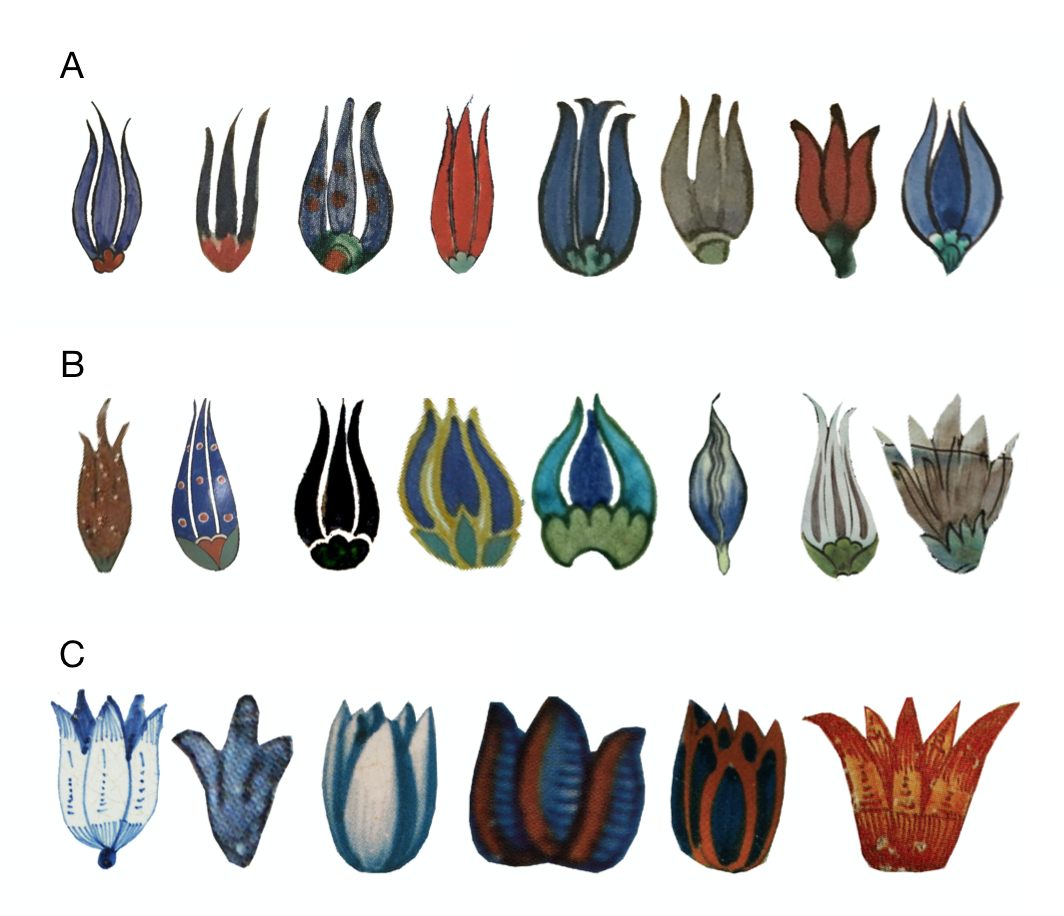
\includegraphics[width=7.5cm]{Proposal/noniznik.png}
\caption{Tulips from artefacts of different stylistic traditions. \textbf{A} ICAROS factory, Rhodos; \textbf{B} Northern European factories; \textbf{C} Dutch Delft}
\label{fig:noniznik}
\end{figure}

\begin{table}[H]
\caption{$AR_{0.5}$, $AP_{0.5}$, and the standard deviation calculated using the ground truth and model predictions on tulips from ICAROS, Northern European factories, Dutch Delft, and Iznik, in three repetitions. Estimated similarity was indicated using $+$ between given stylistic traditions and Iznik}
\centering
\begin{tabular}{ccccc} 
\hline
\multirow{2}{*}{Stylistic  traditions} & \multirow{2}{*}{Similarity to Iznik} & $AP_{0.5}$ & $AR_{0.5}$ \\ 
& & Mean(SD) & Mean(SD) \\ 
\hline
ICAROS & $+++$ & 69.1(2.36) & 78.9(2.60)\\ 
Northern European factories & $+$ & 28.2(4.25) & 48.6(5.70)\\ 
Dutch Delft & $+$ & 48.7(10.6) & 75.9(4.46)\\ 
Iznik &  & 73.7(3.08) &  87.0(4.62) \\ 
\hline
\end{tabular}
\label{tab:similaritytest}
\end{table}
Given these relationships, we expected that our model would be good at identifying Rhodes tulips, do less well at identifying their more distant European-art relations, and be poor at identifying unrelated Delft tulips. As seen in Table \ref{tab:similaritytest}, the model behaved well at identifying ICAROS tulips and did less well at identifying tulips from Northern European factories and Dutch Delft. The model's performance corresponded with the stylistic similarity of each dataset to Iznik, indicating the model could indeed be used for estimating the relationships between different traditions.\par


\section{Discussion}
This project developed and tested a series of computational methods utilising quantitative features like colours, shapes, and relative sizes for the study of Iznik ornaments, and laid the foundation of doing such studies at scale efficiently. \par
I began by developing a method to determine the palette used by Iznik artisans and assigning its colours to individual objects. This method, which was based on sequential clustering of pixel colour values, yielded a result that is generally consistent with the expert palette. However, my method is much more flexible since it does not require expert input and allows the granularity of the discovered palette to be controlled at several levels: object, image and global. This flexibility allows for different palettes to be discovered as needed for different purposes. \par
Using the discovered palettes as well as size and shape descriptors, I analysed the motifs themselves using spectral clustering, a graph-based method that allows clustering even when groups are not Gaussian distributed in high-dimensional space. The resulting lexicon of motifs will, in turn, enable a future analysis on the grammar of Iznik style --- how they are arranged across different artefacts. Rarefaction analysis was also conducted to predict the richness of motifs in tulips. Surprisingly, I found that my sample appears to contain nearly all of the motifs that were made by Iznik artisans. However, as noted, this is only true if my sample is indeed a random sample of the larger population. \par
These results lay the foundation for a future larger study of ornament. They do not, however, solve a basic problem: that there are so many artefacts and ornamental objects. For this reason, I investigated the possibility of using deep learning methods to automatically segment ornamental objects. I showed that a Mask R-CNN based solution could automatically segment and extract motifs out of images to an acceptable quality level, which greatly eases the pain of labour-intensive data collection and preparation for such studies. \par
As usual for deep learning models, my model did not capture all the objects on a given image. In particular, I found that my model performed relatively poorly on saz-leaves, especially when they are clustered together, overlapping with each other, or when an annotated saz-leaf is, in fact, two separate leaves combined together. On the other hand, my results show that the model has the ability to capture the majority of objects, even though they are remarkably diverse in shape (Figure \ref{fig:segmented}). \par
Since the result would be greatly influenced by the representativeness of the training set relative to the wider population, a balanced and well-distributed training set, working as a good sampling of the population that is about to submit to the classification process is needed \parencite{yang2010testing}. Recent studies also found problems in default image augmentation methods like ``flip", arguing it actually changes the feature distribution, which, in turn, mess up tasks that heavily rely on patterns of objects \parencite{lin2020visual}. This calls for a more in-depth look at the data collection and annotation process, as well as a lot more efforts in preparing the training set. A newly proposed Dynamic R-CNN \parencite{zhang2020dynamic} is worth looking  into as it solves the problem of inefficient usage of high-quality samples due to the conflict of fixed settings and the dynamic training procedure. The dynamic $IoU$ and loss function of Dynamic R-CNN is tested to be working well with instance segmentation tasks, improving the performance without adding complexity. Studies have shown promising results in training using a synthetic data set, which allows greater control over the training data in use \parencite{varga2003generation, allken2019fish}. These studies provide a good starting point on improving the performance of our method.\par
Because a deep learning model is trained based on the training set's distinct features, a given model trained on Iznik ornaments naturally learned the stylistic features of them. Hence, the model is also useful when it comes to indicating the similarities between other stylistic traditions and Iznik, that is, to study the evolutionary relationships of the motifs that are \emph{homologous}. It is a pity that only ex-post-facto reasoning can be given due to the nature of neural networks being more or less a black box, hence limiting our ability to explore further to understand why and how it could work better in our favour. Although recent development in explainable artificial intelligence, especially in biology, might be able to tell more on what is going on inside the box and allow us to design a more accurate and controllable tool \parencite{samek2017explainable, ghosal2018explainable}. However, using this method, a test on tulips from ICAROS, Northern European factories, and Dutch Delft ornaments showed that the model is working well, at producing promising results at determining the similarities between their style and that of Iznik. \par
Even though a lexicon of Iznik ornaments can be built, due to the limitation of the dataset used (photographic errors, relatively small amount of data, not enough metadata, etc.), far too little of the information was incorporated to draw any convincing conclusion about their relationships, and it is hard to explain why certain motifs are similar or different from each other, unless with bits of help from archaeology or historical evidence. However, it is easy to see how statistical analyses of the properties of many motifs, their co-occurrence, and their geometrical relationships, could yield a robust classification naturally. \par
In this study, I only sought to lay the methodological foundations for a future study of Iznik ornament. One reason that these data cannot be directly used in evolutionary studies is that most of the artefacts studied here were not dated (They are isolated domestic artefacts.)  That, however, is not true for most Iznik ceramics. Istanbul's Ottoman buildings are covered with thousands of painted Iznik tiles and, since the construction dates of these buildings are known, the manufacture dates of their tiles are --- with some qualifications --- known too. These tiles, as well as a handful of convincingly dated pots and plates, if studied using our methods, could form the basis of a statistical model of the evolution of Iznik design. Another way of gathering such metadata is through computational methods, in fact, it has already been done on identifying authors and painters and showing promising results \parencite{qian2017deep, widjaja2003identifying}.\par
It is the transmission of these motifs that is fascinating, and the ultimate goal is the construction of a comprehensive library of training sets and models based on many ornamental traditions that will permit the construction of a genealogical network of ornamental styles that spans cultures, centuries and continents. Since all these methods are computational and automated, it should be possible to scale them up to facilitate such studies.\par
Finally, returning to Darwin, I note that, although I have studied cultural ornaments, there is no reason that these methods cannot be applied to those found on living things. It would, for example, be relatively easy to use the methods I have developed to study the evolution of ornament of bird plumage --- of which the Argus pheasant is only one spectacular example.\par
\subsection*{Data and code availability}
All data and codes used can be found on the \href{https://github.com/gregiee/CMEEcoursework/tree/master/ThesisProject}{project github}.

%%TC:ignore
\clearpage
\printbibliography
\clearpage


\setcounter{table}{0}
\renewcommand{\thetable}{S\arabic{table}}
\setcounter{figure}{0}
\renewcommand{\thefigure}{S\arabic{figure}}


\section{Supplementary Information}
\subsection{Tables}
\begin{table}[H]
\caption{Types of artefacts and counts}
\small
\centering
\begin{tabular}{cccc} 
 \hline
Artefact type & Count & Artefact type & Count \\ 
\hline
Candlestick & 1 & Plate & 367 \\ 
Jar & 1 & Spandrel & 6\\ 
Jug & 15 & Tankard & 14\\ 
Mosque lamp & 1 & Tile & 151\\ 
Panel & 8 & Vase & 6\\ 
Basin & 5 & Total & 575 \\ 
\hline
\end{tabular}
\label{tab:artefacttype}
\end{table}

\begin{table}[H]
\caption{Training and testing set of each repetition of the instance segmentation task}
\small
\centering
\begin{tabular}{ccccccc} 
\hhline{~~-----}
 & & Saz-leaf & Carnation & Tulip & Total & Image count \\ 
\hline
\multirow{2}{*}{Repetition 1} & Train & 1593 & 448 & 1782 & 3823 & 515\\
\hhline{~~~~~~} & Test & 163 & 56 & 263 & 482 & 60\\
\hhline{~------}
\multirow{2}{*}{Repetition 2} & Train & 1612 & 463 & 1731 & 3806 & 515\\
\hhline{~~~~~~} & Test & 144 & 41 & 314 & 499 & 60\\
\hhline{~------}
\multirow{2}{*}{Repetition 3} & Train & 1586 & 448 & 1871 & 3905 & 515\\
\hhline{~~~~~~} & Test & 170 & 56 & 174 & 400 & 60\\
\hline
\end{tabular}
\label{tab:repetition}
\end{table}


\subsection{Figures}
\begin{figure}[H]
\centering
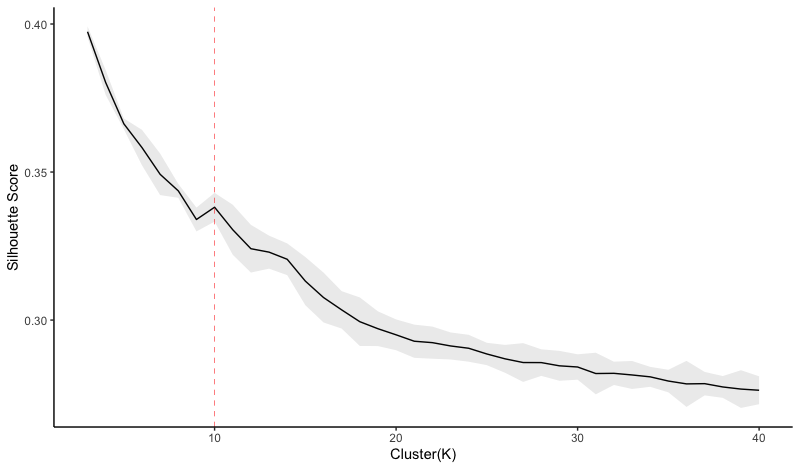
\includegraphics[width=14cm]{Proposal/silscore.png}
\caption{Silhouette score curve with standard deviation in ribbon shades of 100 repetitions of k-means clustering, K=[2,40]. A local optimal can be seen at K=10}
\label{fig: silscore}
\end{figure}


\begin{figure}[H]
\centering
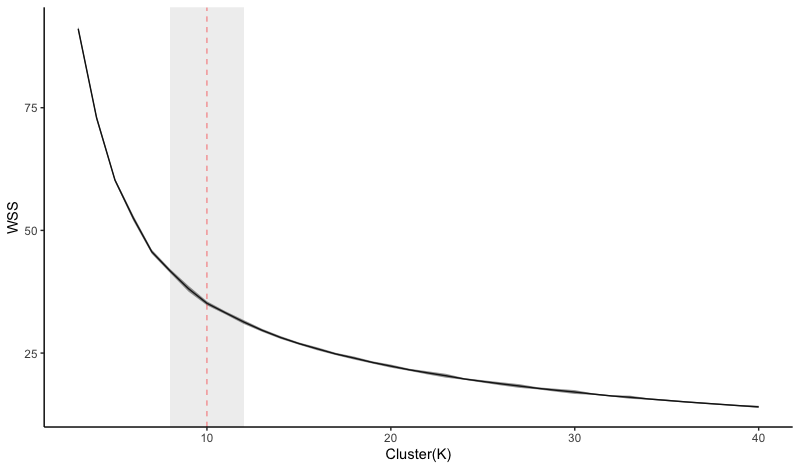
\includegraphics[width=14cm]{Proposal/wss.png}
\caption{Within-cluster sum of square (WSS) curve with standard deviation in ribbon shades of 100 repetitions of k-means clustering, K=[2,40]. An elbow is estimated to be in the gray box around K=10}
\label{fig: wss}
\end{figure}

\begin{figure}[H]
\centering
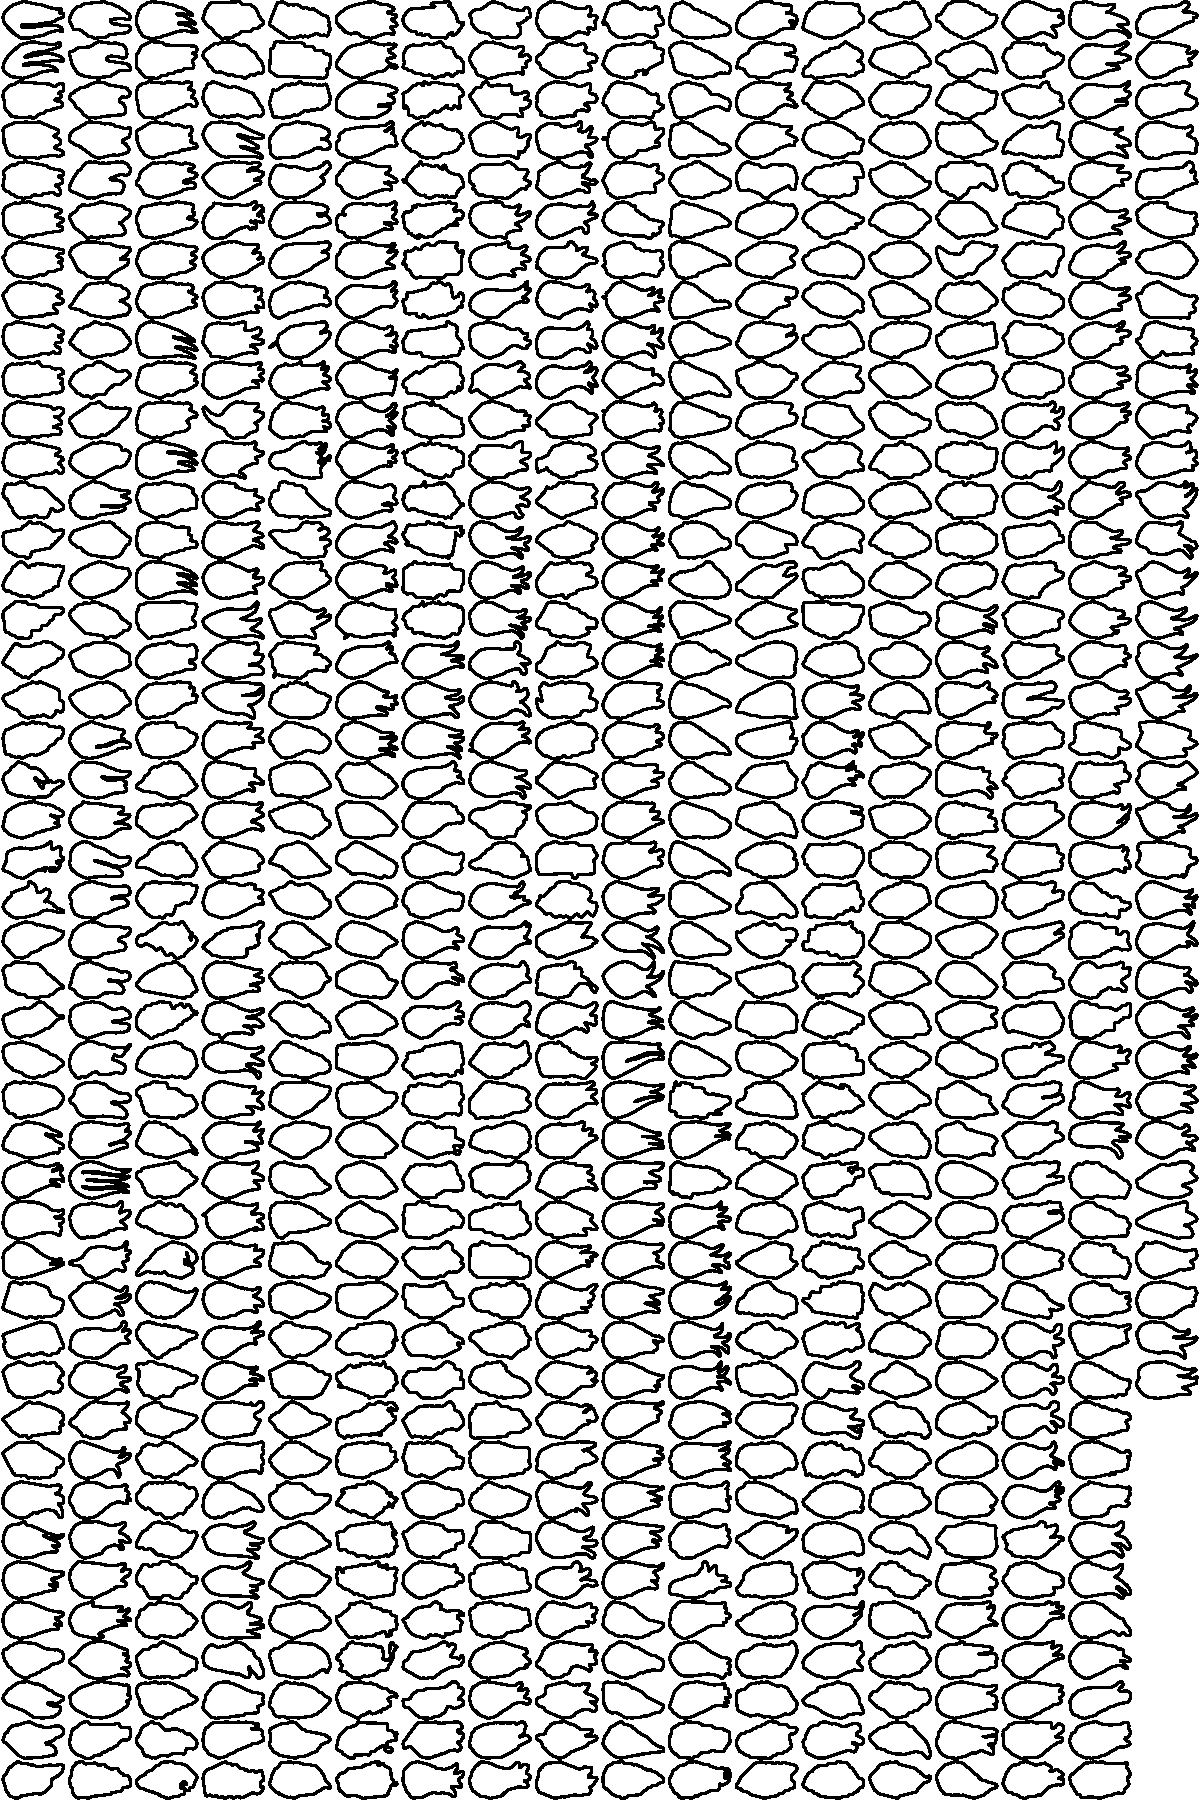
\includegraphics[width=16cm]{Proposal/alignedtulip.pdf}
\caption{Part of the standardised tulips used for lexicon discovery, aligned using the method proposed in this study}
\label{fig:alignment}
\end{figure}

\begin{figure}[H]
\centering
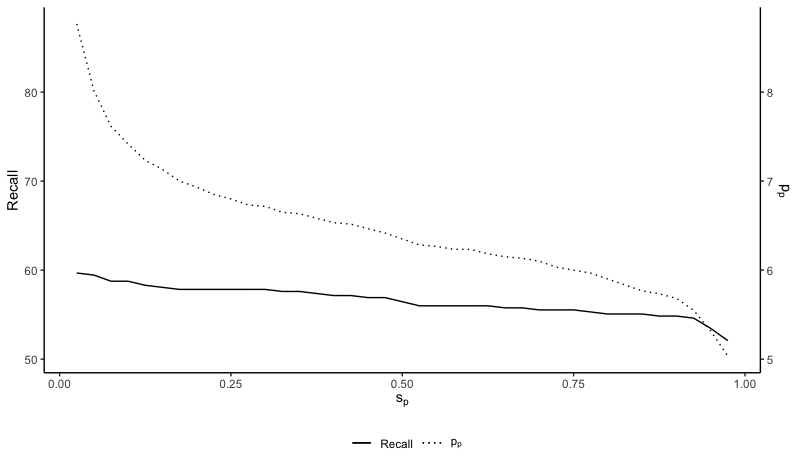
\includegraphics[width=14cm]{Proposal/recall.png}
\caption{$Recall$ and remaining prediction percentage, $p_{p}$ against prediction score, $s_{p}$, with an $IoU$ threshold of 0.75 }
\label{fig: recall}
\end{figure}

\begin{figure}[H]
\centering
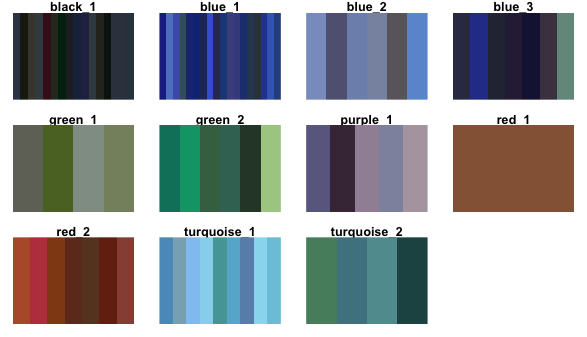
\includegraphics[width=14cm]{Proposal/expertpal.png}
\caption{Colours picked from sample images to aggregate the 11 colour Expert palette. Level of abstraction is not consistent, colour variation is vastly different, and there are some human errors in picking the colours, especially in $black_1$ }
\label{fig:expertpalproblem}
\end{figure}

\begin{figure}[H]
\centering
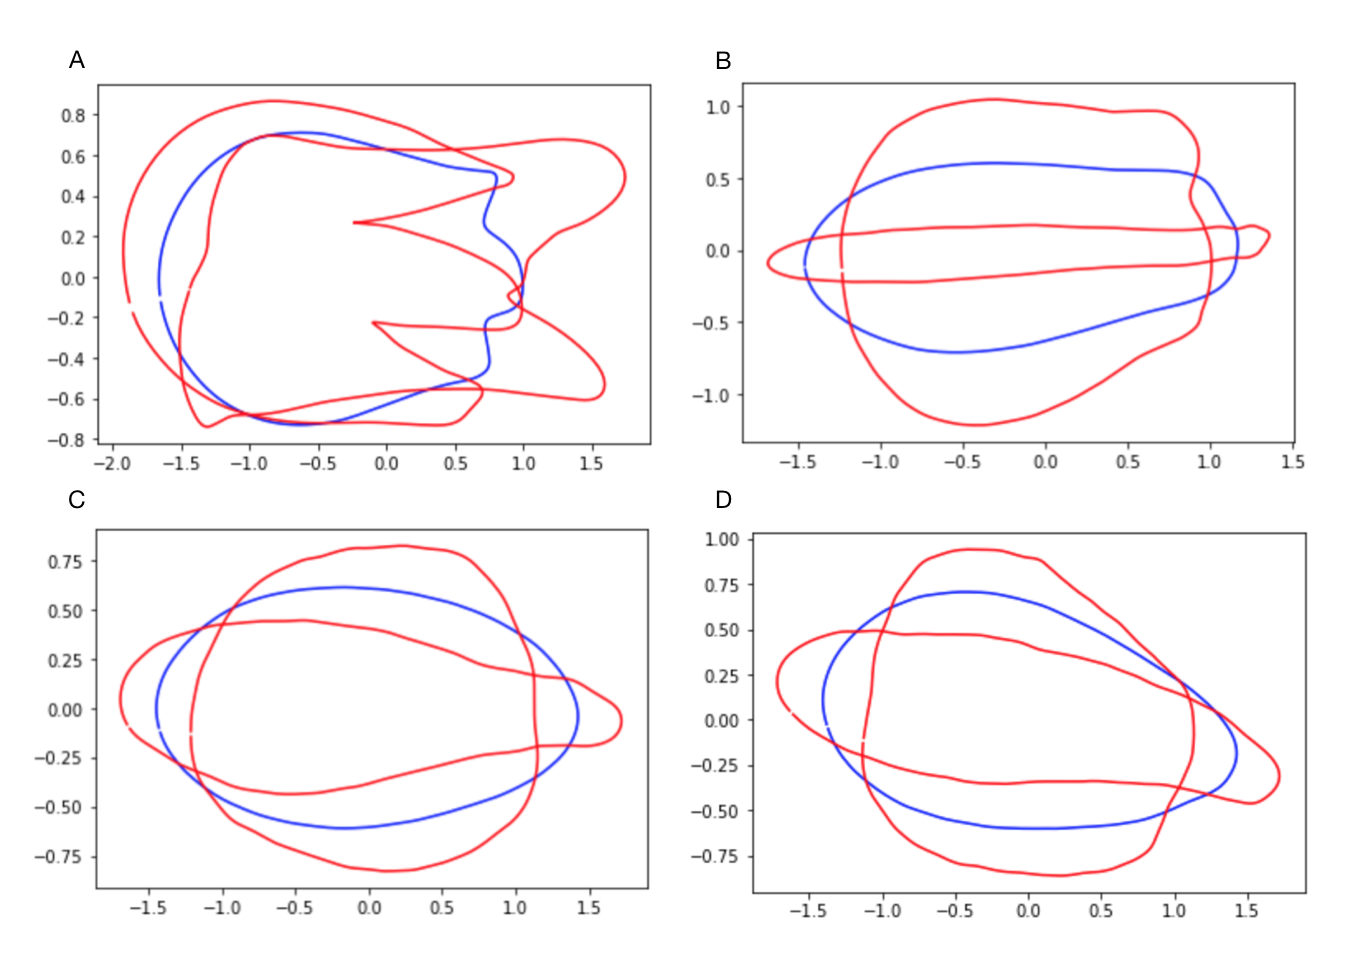
\includegraphics[width=14cm]{Proposal/shaperesult.png}
\caption{Cluster results on shape, with blue line indicate the mean shape with in a cluster, red lines indicating the standard deviation, applied with first eigen vectors. \textbf{A} cluster 1; \textbf{B} cluster 2; \textbf{C} cluster 3;  \textbf{D} cluster 4}
\label{fig:clustershape}
\end{figure}

\begin{figure}[H]
\centering
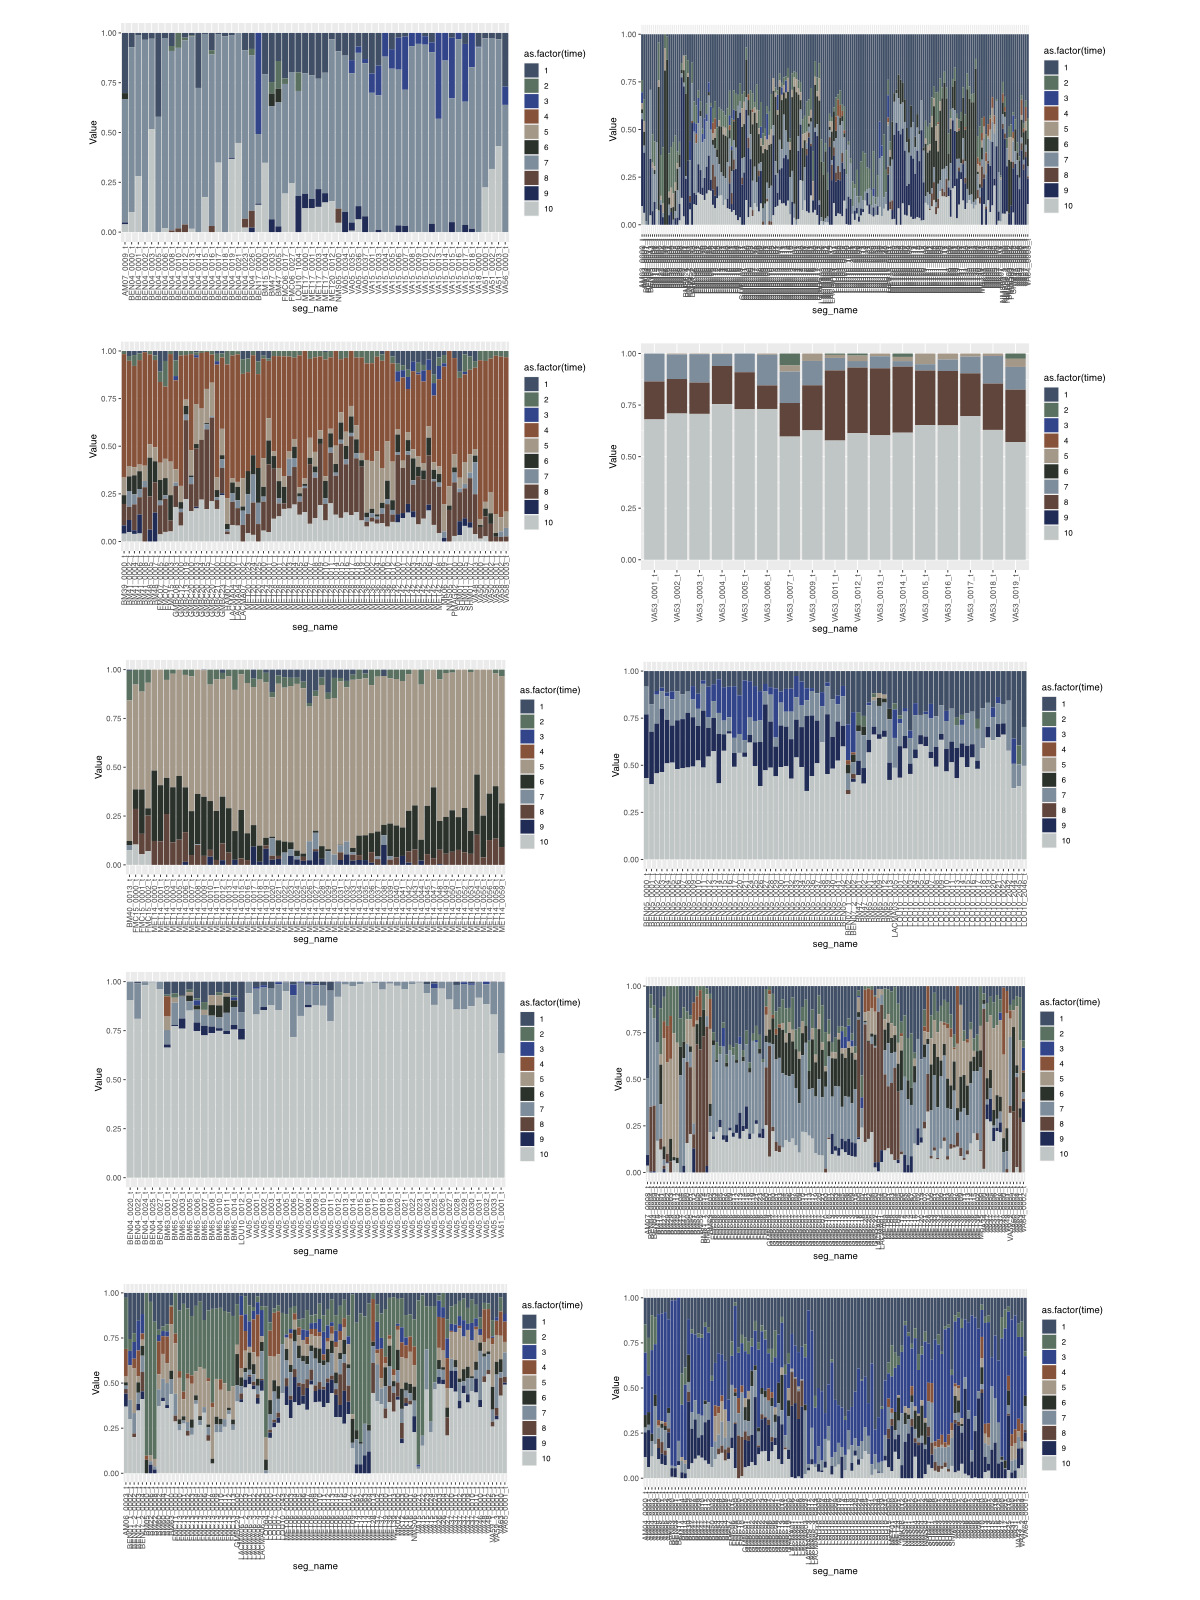
\includegraphics[width=18cm]{Proposal/colourresult.jpeg}
\caption{Cluster results on colour. Each sub-plot represent a cluster, and is of each tulip's colour palette and its corresponding frequency}
\label{fig:clustercolour}
\end{figure}

\subsection{Defining motifs}
\label{sec:definemotifs}
It is easy to pick out ideal Iznik representations of tulip, carnation and saz-leaf, however, a comprehensive survey of decorative motifs shows many deviations from the ideal. Iznik artisans painted many different kinds of flowers and leaves, but since they didn't care very much about botanical accuracy, it can be be hard to identify which species they had mind as they picked up their brushes. When constructing the training set, operational definitions were introduced to help pick out motifs.

\subsubsection*{Tulip}

A ``tulip'' is defined as an representation of a petaloid monocot (tulips, daffodils, lilies \emph{etc}) flower with the following properties:
\begin{enumerate}
\item lateral (rather than corolla) view.
\item distal-proximal (base-tip) axis typically greater than left-right axis.
\item simple, oblate, petals.
\item sepals that do not embrace the flower or exceed its distal margin. This excludes ``rose buds''.
\item a corolla with a maximum diameter midway along the proximal-distal axis rather than distally (i.e., tulip- rather than cup-shaped). This excludes [what] 
\item single flower per stem. This excludes ``campanulas'' which are represented as having many flowers coming from a single stem.
\item leaves, if present, are cauline and strap shaped. They are not segmented.
\end{enumerate}

\subsubsection*{Carnations}

A ``carnation'' was defined an representation of a flower many, not necessarily all, of the following features:

\begin{enumerate}
\item lateral (rather than corollar) view. Carnations are frequently depicted from a corollar view, but these were exclude.
\item multiple petals.
\item lobate petals.
\item red colour.
\item calyx with a maximum diameter midway along the proximal-distal axis rather than distally (i.e., tulip- rather than cup-shaped)
\item sepals that do not embrace the flower or exceed its distal margin. This excludes ``rose buds''.
\item has a pair of anthers protruding beyond the corolla.
\end{enumerate}
\subsubsection*{Saz-leaf}

A ``serrated leaf'' is is a leaf that has the following features, not all of which need be present:
\begin{enumerate}
\item acicular (needle) shape, that is, with a distal-proximal (base-tip) axis greater than left-right axis
\item a rachis (``spine'').
\item serrate or lobulate margins. 
\item isolated, though they may overlap or inter-penetrate or be arranged in a basal rosette (as in a dandelion). 
\item twisted into a simple curve or s-shape.
\item depicted from a partial lateral, rather than a dorsal or ventral, view so that the blade of the leaf is on one side of the rachis.
\item multi-coloured.
\item If compound (composed of many leaflets emerging from a rachis), then the entire unit, rather than the individual leaflets, is considered as a ``serrated leaf''.
\item If two more leaves are fused (without a stem between them) then the entire unit is considered a single ``serrated leaf''; if separated by a stem then they are considered as separate ``serrated leaves''.
\item The following leaves are not counted as ``serrated leaves'':
\begin{enumerate} 
\item leaves attached to a stem (as in a rose-bud),
 \item an appendage to a larger ornamental motif such as a rosette, 
 \item tulip leaves.
 \end{enumerate}
\end{enumerate} 
%%TC:endignore
\end{document}